%%%%%%%%%%%%%%%%%%%%%%%%%%%%%%%%%%%%%%%%%%%%%%%%%%%%%%%%%%%%%%%%%%
%%%%%%%% ICML 2015 EXAMPLE LATEX SUBMISSION FILE %%%%%%%%%%%%%%%%%
%%%%%%%%%%%%%%%%%%%%%%%%%%%%%%%%%%%%%%%%%%%%%%%%%%%%%%%%%%%%%%%%%%

% Use the following line _only_ if you're still using LaTeX 2.09.
%\documentstyle[icml2015,epsf,natbib]{article}
% If you rely on Latex2e packages, like most moden people use this:
\documentclass{article}

% use Times
\usepackage{times}
% For figures
\usepackage{graphicx} % more modern

%H
%\usepackage{caption}
%\usepackage{subcaption}

%\usepackage{epsfig} % less modern
%\usepackage{subfigure} 

% For citations
\usepackage{natbib}

% For algorithms
\usepackage{algorithm}
\usepackage{algorithmic}

% As of 2011, we use the hyperref package to produce hyperlinks in the
% resulting PDF.  If this breaks your system, please commend out the
% following usepackage line and replace \usepackage{icml2015} with
% \usepackage[nohyperref]{icml2015} above.
\usepackage{hyperref}

% Packages hyperref and algorithmic misbehave sometimes.  We can fix
% this with the following command.
\newcommand{\theHalgorithm}{\arabic{algorithm}}

\usepackage{amsmath,amsfonts,amssymb,amsthm}

% Employ the following version of the ``usepackage'' statement for
% submitting the draft version of the paper for review.  This will set
% the note in the first column to ``Under review.  Do not distribute.''
\usepackage{icml2015} 

% Employ this version of the ``usepackage'' statement after the paper has
% been accepted, when creating the final version.  This will set the
% note in the first column to ``Proceedings of the...''
%\usepackage[accepted]{icml2015}


% The \icmltitle you define below is probably too long as a header.
% Therefore, a short form for the running title is supplied here:
\icmltitlerunning{Symbolic Gibbs Sampling in Piecewise Algebraic Graphical Models with Nonlinear Deterministic Constraints}

\usepackage{verbatim}
%\usepackage{ntheorem} % framed and list of theorems [standard,framed,thref] \listtheorems{types}		%COMMENTED BY HADI
\usepackage{color}    % color
\newtheorem{theorem}{Theorem}

%OLD
\newcommand{\fix}{\marginpar{FIX}}
\newcommand{\new}{\marginpar{NEW}}
\newcommand{\ind}[1]{\mathbb{I}[#1]}
\newcommand{\inde}{\mathbb{I}}

\newcommand{\var}{v}
\newcommand{\eq}{\leftarrow}

\newcommand{\LB}{\mathit{LB}}
\newcommand{\UB}{\mathit{UB}}

\newcommand{\B}{\mathbb{B}}
\newcommand{\E}{\mathbb{E}}
\newcommand{\I}{\mathbb{I}}
\newcommand{\R}{\mathbb{R}}

\newcommand{\F}{\mathbb{F}}
\renewcommand{\vec}[1]{\mathbf{#1}}

%NEW:
\newcommand{\tuple}[1] {\langle #1 \rangle}
\newcommand{\bvec}[1]{\textbf{#1}}
\newcommand{\indicator}{\mathbb{I}}%{I\!\!I}
\newcommand{\case}[2]{#2 &\text{ if } #1}%{#1 : #2}
\newcommand{\singlecase}[2]{#2 \quad \text{ if } #1}
\newcommand{\otherwise}[1]{#1 &\text{ otherwise}}
\newcommand{\pr}{p}
\newcommand{\nn}{0.16}


\begin{document} 

\twocolumn[
\icmltitle{Symbolic Gibbs Sampling in Piecewise Algebraic Graphical Models with Nonlinear Deterministic Constraints}

% It is OKAY to include author information, even for blind
% submissions: the style file will automatically remove it for you
% unless you've provided the [accepted] option to the icml2015
% package.
\icmlauthor{Your Name}{email@yourdomain.edu}
\icmladdress{Your Fantastic Institute,
            314159 Pi St., Palo Alto, CA 94306 USA}
\icmlauthor{Your CoAuthor's Name}{email@coauthordomain.edu}
\icmladdress{Their Fantastic Institute,
            27182 Exp St., Toronto, ON M6H 2T1 CANADA}

% You may provide any keywords that you 
% find helpful for describing your paper; these are used to populate 
% the "keywords" metadata in the PDF but will not be shown in the document
\icmlkeywords{Deterministic, evidence, relations, constraints, random variables, Symbolic, Analitical, Gibbs sampling}

\vskip 0.3in
]

\begin{abstract}
In many applications of probabilistic reasoning, there are deterministic relationships between
continuous random variables. These relationships create serious problems for approximate or exact inference.
%Such deterministic conditionals create serious problems for exact or approximate inference.
To avoid the complications, algorithms such as \emph{Bayesian inference using Gibbs sampling} (BUGS) simply disallow such dependencies.  
%For example, in BUGS it is impossible to model observed data that is the sum of two random variables. 
There are no known exact or Monte Carlo inference methods that can handle deterministic constraints beyond the limit of linear dependencies.
%Many classes of conjugate distributions %such as \emph{conditional linear Gaussians} 
%can handle linear deterministic conditionals. 
%General purpose full automated inference in the presence of non-linear deterministic constraints, however, is beyond the scope of the existing conjugate solutions and Monte Carlo algorithms.    
In this paper we fill this gap by contributing a novel framework which,
for the first time, carries out inference in models with nonlinear algebraic deterministic constraints. % that are not discussed in the literature so far.
Our second contribution is to provide an effective MCMC inference technique called \emph{Symbolic Gibbs}, based on the insight that in our model, most costly operations required for Gibbs sampling can be accomplished offline and prior to sampling. 
We evaluate this algorithm on models in physics and engineering and show that it is an order of magnitude faster than the baseline Gibbs sampler and a significant improvement over other Monte Carlo methods.  
\end{abstract}

\section{Introduction}
\label{sect:intro}
Graphical models (GMs) are the lingua franca for probabilistic reasoning.
They denote the conditional dependence structure between random variables by directed or undirected graphs \cite{koller2009probabilistic}. A (random) variable is deterministic if its conditional distributions have zero variances. 
%Unobserved deterministic random variables that is, variables that cannot be given data or initial values (corresponding to \emph{logical nodes} in BUGS software) almost only provide notational convenience.
Observed deterministic variables represent deterministic dependencies on other variables.
Such constraints can appear in a variety of real-world applications.
For instance, instead of direct observation of random variables 
$X_1, X_2, \ldots$, a function of them $f(X_1, X_2, \ldots)$ might be observed. 
%such deterministic relationships between random variables might be governed by natural laws (such as Kirchhoff's circuit laws or Newtonian mechanics).

To motivate the discussion consider a concrete example:  
%%%%%%%%%%%%%%%%%%%%%%%%%%%%%%%%%%%%%%%%%%%%%%%%%%%%%%%%%%%%%%%%%%%%%%%%%%
%%%%%%%%%%%%%%%%%%%%%%%%%%%%%%%%%%%%%%%%%%%%%%%%%%%%%%%%%%%%%%%%%%%%%%%%%%
\begin{figure}
\begin{center}
\begin{minipage}{\linewidth/6}
%\begin{center}
%\vspace{-1mm}
%\quad
%\begin{subfigure}{0.19\linewidth}
                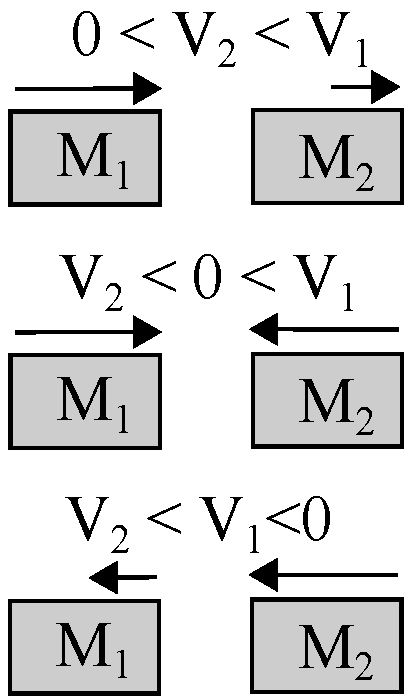
\includegraphics[width=1\linewidth]{Figs/little-momentum0.pdf}
               %\\		\begin{center}(b)\end{center}%\caption{}
              %\label{fig:mom0}
%    \end{subfigure}%
\end{minipage}
\hspace{7mm}
\begin{minipage}{\linewidth/2}
%\qquad
%\begin{subfigure}{0.52\linewidth}
                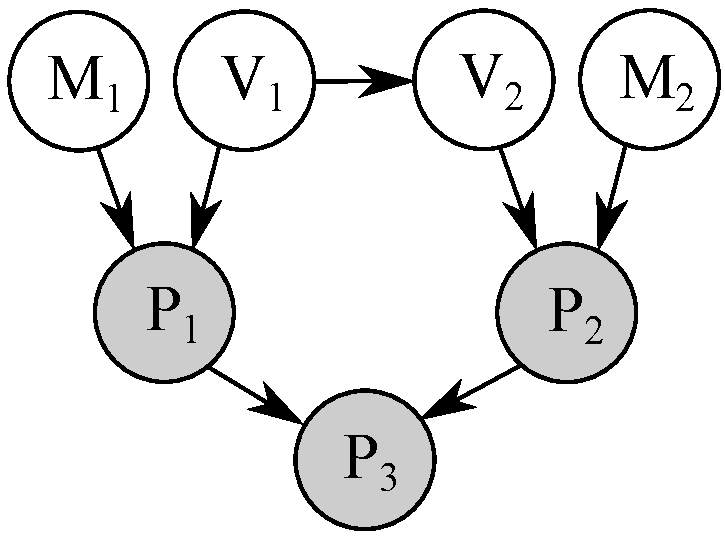
\includegraphics[width=0.80\linewidth]{Figs/little-momentum1.pdf}
                %\\		\begin{center}(b)\end{center}%\caption{}
                %\label{fig:mom00}
    %   \end{subfigure}%
%\end{center}
\end{minipage}
\vspace{3mm}\\
(a) \hspace{30mm}(b)
%\vspace{-1mm}
\caption{\footnotesize 
Collision of masses $M_1$ and $M_2$ with velocities $V_1$ and $V_2$ and momenta $P_1$ and $P_2$. 
(a) Collision happens if and only if $V_1>V_2$. (b) Corresponding Bayesian network. The non-filled and filled Filled circles represent stochastic and deterministic random variables respectively.} 
\label{fig:mom0}
\vspace{-4mm}
\end{center}
\end{figure}
%%%%%%%%%%%%%%%%%%%
%%%%%%%%%%%%%%%%%%%
%\vspace{1mm}\\
{\bf Example (Collision model). }
\emph{Masses $M_1$ and $M_2$ with velocities $V_1$ and $V_2$ (and consequently momenta $P_1 = M_1 V_1$ and $P_2 = M_2 V_2$) collide to form a single mass ($M_1 + M_2$) with momentum $P_3 = P_1 + P_2$ (assuming that there is no dissipation).
Masses and velocities are unknown but 
their prior distributions are given as follows\footnote{
$Throughout, \mathcal{U}(a, \, b)$ denotes a uniform continuous distribution 
with {\color{green} support interval} $[a, b]$.
} 
(note that as Figure~\ref{fig:mom0}.a shows, a collision only happens if $V_2 < V_1$):  
}%end \emph
\begin{align}
&\pr(M_1) = \mathcal{U}(0.1, \, 2.1) 
&&\pr(M_2) = \mathcal{U}(0.1, \, 2.1)
\nonumber
\\
&\pr(V_1) = \mathcal{U}(-2, \, 2)
&&\pr(V_2 \, | \, V_1) = \mathcal{U}(-2, \, V_1)
\label{e:collision}
\end{align} 
\emph{
The conditional dependencies of these random variables are illustrated in 
Figure~\ref{fig:mom0}.b.
Conditioned on the observation $P_3 = 3$, the posterior joint distribution of $M_1$, $M_2$, $V_1$ and $V_2$ is desired. 
\hspace*{\fill} $\diamond$} %\emph

Despite its humble appearance, the solutions that the existing probabilistic inference tools provide for this model are quite unsatisfactory. 
As a matter of fact, we are unaware of any existing general inference framework that 
handles observed deterministic relationships between random variables!\footnote{
By imposing various (but functionally the same)
\emph{syntactical restrictions} and excuses, 
the state-of-the-art probabilistic programming toolkits
totally disallow deterministic relationships among continuous random variables be observed:
In BUGS \cite{lunn2009bugs}, the popular software for analysis of statistical models, \emph{logical nodes} cannot be given data or initial values .
In PyMC \cite{patil2010pymc} deterministic variables have no \emph{observed flag}. 
If in Stan {\color{red}TODO cite} 
you try to assign an observation value to a deterministic variable, you will encounter an error message: 
``attempt to assign variable in wrong block'' while 
Anglican{\color{red} TODO cite} throws error ``invalid-observe", etc.}

Let's take a closer look on the nature of the problem by manually carrying on the computations required for MCMC sampling:
It can easily be seen that in the \emph{collision model}, 
the \emph{prior} joint probability of 
{\footnotesize $M_i$} and 
{\footnotesize $V_i$} is:
{\footnotesize
\begin{equation}  
\label{e:col-prior}
\pr(M_1, M_2, V_1, V_2)  
=
\begin{cases}
\frac{1}{16 V_1 + 32} &{\text{if }\scriptstyle 0.1<M_1<2.1, \, 0.1<M_2<2.1,}\\
							 &{\;\;\, \scriptstyle -2<V_1<2, \, -2<V_2 < V_1}\\
 \otherwise{0}
 \end{cases}
\end{equation}
}
which is a 4 dimensional function from which samples can be taken fairly easily. 
Since {\footnotesize $P_3 = M_1 V_1 + M_2 V_2$}, 
the following \emph{likelihood} is a 0-variance conditional distribution:
\begin{equation}
\label{e:col-likelihood}
\pr(P_3 = 3 \,|\, M_1, V_1, M_2, V_2) = \delta[3 - (M_1 V_1 + M_2 V_2)]
\end{equation}
where $\delta[\cdot]$ denotes \emph{Dirac delta}. 
By \emph{Bayes} rule, 
the \emph{posterior} 
{\footnotesize $\pr(M_1, M_2, V_1, V_2 \,|\, P_3 = 3)$}
is proportional to the product of equations (\ref{e:col-prior}) and (\ref{e:col-likelihood}) 
that despite being a 4-dimensional function, its mass is only non-zero on the 3 dimensional \emph{hypersurface}: {\footnotesize$M_1 V_1 + M_2 V_2 = 3$}. 


In general, observation of an algebraic function of an $N$-dimensional prior often leads to a posterior mass positioned on an $N-1$-dimensional hyperspace and existence of more deterministic constraints/relationships between stochastic random variables increases the difference between the dimensionality of the original space and the \emph{manifold} on which the posterior is non-zero.  
If this dimensionality mismatch is not taken into account, sampling from such posterior distributions via sampling is impossible.\footnote{As a more tangible example, note that taking sample from a 2D curve via random walk in a 3D continuous space is impossible.}  

The solution that the existing MCMC-based frameworks suggest is to approximate the observed deterministic relations among  stochastic random variables via adding noise to the observation 
(hard to soft constraint conversion by introducing measurement error).

For example the r.h.s of equation (\ref{e:col-likelihood}) would be 
approximated with a normal distribution
{\footnotesize $\mathcal{N}(3 - M_1 V_1 - M_2 V_2, \sigma_\eta)$}  
where the standard deviation $\sigma_\eta$ is the noise parameter.

Using this trick, it is guaranteed that the posterior is equidimensional with the (space of) prior (i.e.\ its ambient space) and therefore in theory, conventional MCMC sampling is possible.
Nonetheless, in practice such an strategy may not help much:
If the added noise is large, 
the approximation bounds may become arbitrarily large
and if the noise is small, 
the mixing rate may become extremely slow \cite{chin1987bayesian}. 
The reason is that in the latter case, 
 the approximated posterior mass would be dense in tinny regions (surrounding the original manifold) on which random walk
is notoriously inefficient (near deterministic problem).  

In particular cases, the problem may be addressed via 
\emph{variable transformations}.
Most notably, 
the family of \emph{conditional linear Gaussians (CLG)} \cite{lauritzen2001stable}
is closed under linear transformations and consequently
allow linear deterministic constraints.
However, inference in the presence of nonlinear deterministic constraints on continuous random variables is still an open problem \cite{li2013dynamic}.
 
In this paper we solve this problem for a large class of nonlinear multivariate algebraic deterministic constraints in the form of polynomial fractions. 

After a brief background for representation and inference in Graphical models (GMs) in Section~\ref{sect:background}, 
our first main contributions is presented in Section~\ref{sect:contribution1}:
{
\bf
We provide an automated algorithm (called \emph{collapsing determinism}) for Bayesian inference in 
presence of observed deterministic algebraic relationships among random variables.
}
%\end{center}

The main idea is to reduce the posterior dimensionality by utilizing 
the properties of Dirac delta distributions. 
This algorithm relies on operations such as fractional substitutions. 
It can easily be seen that under such operations, the typical classes of distributions that are studied in the literature so far do not remain closed.
This should be the main reason why the problem of inference conditioned on determinism has remained {\color{green}untackled} so far. 

Our second contribution is presented in Section~\ref{sect:ppfs} where we {\color{green}alleviate} this situation as follows:
{\bf
We introduce an extremely expressive class of distributions with properties that facilitate the inference conditioned on deterministic algebraic constraints.
}

This class (called PPFs for \emph{polynomial piecewise fractions}) {\color{green}consists of} piecewise functions where the space of variables is partitioned by polynomial inequalities and the the function value in each partition is a fraction with a polynomial numerator and denominator.  
%Clearly, PPFs can approximate any function up to arbitrary precision by partitioning it into (relatively) {\color{green} homogeneous} pieces followed by utilizing \emph{Taylor} expansion or similar methods.
The key insight is that PPFs are closed under derivation and polynomial fractional substitutions. This immediately extends their application to models with sophisticated algebraic constraints.

Unfortunately, PPFs are not closed under integration 
(required for marginalization).
Therefore, closed-form inference on PPF models is not in general possible. 
Nonetheless, a large subset of PPFs have closed-form univariate symbolic integrals which lead to our third major contribution that is offered in Section~\ref{sect:symbolic.gibbs}:
{
\bf
Presenting an efficient asymptotically unbiased inference method (called \emph{Symbolic Gibbs}) that matches well with PPF models and the provided algorithm for conditioning on determinism.
}

%The second contribution, as mentioned, is a new variation of Gibbs sampling.  
Gibbs samplers are robust in the sense that they do not need any parameter tuning.
However, they are computationally expensive since to take a single sample they require to compute many univariate integrals (to generate the CDFs of conditional distributions).
%We notice that a large subset of PPFs have closed form (symbolic) integrals. 
The idea of Symbolic Gibbs is to compute a single analytic integral for each variable by keeping the remaining variables uninstantiated. 
The actual process of CDF computation per sample  
simply involves instantiation of the already computed CDFs rather than computing them on the fly.
This dramatically decreases the amount of necessary computations and as in Section~\ref{sect:experimental.results} the experimental results show, leads to a significant performance improvement. 

Literature review is postponed to Section~\ref{sect:literature.review} and Section~\ref{sect:conclusion} concludes. 

%In the following sections after a brief introduction to Graphical models, followed by an algorithm for inference in the presence of deterministic constraints.We then explain the restrictions of PPFs, compare our method with other samplers and conclude. 

\section{Graphical Models (GMs)}
\label{sect:background}
Let $\vec{X} = \{X_1, X_2, \ldots\}$ be a set of random variables with realizations in the form 
$\vec{x} = \{x_1, x_2, \ldots\}$.\footnote{
As a common abuse of notation, in case there is no ambiguity, we do not distinguish between random variables and their realizations; e.g., we abbreviate $\pr(X_i = x_i)$ with $\pr(x_i)$.}
$\vec{X}$ may contain discrete and continuous variables. 
However, for the sake of notational consistency, %and since the problems tackled in this paper only hold for continuous variables, 
we only consider continuous models throughout. 
Note that inference in presence of discrete deterministic constraints is trivial.
Therefore, generalization of the presented framework to hybrid discrete/continuous models is straightforward.   

To cover both directed and undirected graphical models we use
\emph{factor graph} notation \cite{kschischang2001factor}
and represent a joint probability distribution $\pr(\vec{X})$ in a factorized form as follows: 
\begin{equation}
\label{e:factor-graph}
\pr(\vec{X}) \propto \prod_{\Psi_k \in \boldsymbol\Psi} \Psi_k (\vec{X}_k)
\end{equation}
where 
$\Psi(\vec{X}_k)$ are a non-negative, real-valued \emph{potential functions} (of a subsets $\bvec{X}_k$ of $\vec{X}$) and the normalization constant is not necessarily known.
Throughout, we adopt the notation 
$\textsc{Scope}(\Psi_k) := \bvec{X}_k$.
%$C$ is a (not necessarily known) normalization constant.
%The inference procedure that will be presented does not require the normalization constant be known. 

\textbf{Inference.}
The inference task studied in this paper is 
the computation of the \emph{posterior} joint distribution 
$\pr(\bvec{Q} \,|\, \bvec{E}=\bvec{e})$
of 
a subset $\bvec{Q}$ of $\bvec{X}$ (\emph{query})
conditioned on (realization $\bvec{e}$ of) 
variables  
$\bvec{E} \subset\bvec{X} \backslash \bvec{Q}$ (\emph{evidence}):
\begin{equation}
\label{e:inference}
\pr(\vec{Q} \,|\, E =\vec{e}) \propto 
\int_{w_1 = -\infty}^{\infty} \!\!\!\!\!\! \cdots \int_{w_m = -\infty}^{\infty}
%\prod_{\Psi \in \boldsymbol\Psi} \Psi(\vec{x})
\!\!\!\!\!\!\!\! \pr(\bvec{Q}, \bvec{W} = \bvec{w}, \bvec{E}=\bvec{e} )
\, d \bvec{w}
\end{equation}
where $\bvec{W} = \{W_1, \ldots, W_m\} := \vec{X} \backslash (\vec{Q} \cup \vec{E})$ and its realization is in form $\bvec{w} = \{w_1, \ldots, w_m\}$.

The main challenge for closed inference is the computation of multiple integrals required for \emph{marginalizing {\color{green}out}} $\bvec{W}$.
There are a few classes of functions which are closed under integration.
However, none of these classes can handle deterministic constraints beyond the level of linear constraints.
\\
\textbf{Monte Carlo methods}
%An alternative to exact inference is to approximate the joint distribution by a set of samples drawn from it using Monte Carlo methods. By the law of large numbers, this approximation is asymptotically unbiased. Using samples, the costly marginalization operation is avoided since the conditional probability $\pr(\bvec{q} \,| \, \bvec{e})$ is simply approximated by the number of samples satisfying $\bvec{q} \cap \bvec{e}$ divided by the number of samples satisfying $\bvec{e}$.
%Note that unlike other approximate methods, inference via sampling leads to asymptotically unbiased solutions i.e.\ by taking sufficient number of samples, the \emph{posterior} can be approximated by an arbitrary precision.
Approximating the posterior distribution via drawing samples from it by Monte Carlo methods 
provides an asymptotically unbiased tool that completely avoids the hassle of multiple integrations.% required in closed-form sampling.   
Three major such methods are as follows:

\emph{Rejection sampling}: In this method, to draw a sample from 
a distribution $p(\bvec{X})$, a sample $\bvec{x}$ is taken from another distribution $q(\bvec{X})$
such that $p(\bvec{X})/q(\bvec{X})$ is bound by a known constant $c$
and samples can be taken from $q(\bvec{X})$ efficiently.
The produced sample is accepted with probability $p(\bvec{x}) / c q(\bvec{x})$, 
otherwise it is rejected and the process is repeated. 

\emph{Metropolis-Hastings (MH)}:
To draw a new sample $\bvec{x}^{(t)}$ from a distribution $p(\bvec{X})$, given a previously taken sample $\bvec{x}^{(t-1)}$, 
MH takes a sample $\bvec{x}'$ from a symmetric \emph{proposal density} $q(\bvec{X} |\, \bvec{x}^{(t-1)})$. 
%from which samples can be taken efficiently 
%(often an isotropic \emph{Gaussian} centered at $\bvec{x}^{(t-1)}$). 
With probability $\min \big(1, p(\bvec{x}')/p(\bvec{x}^{(t-1)}) \big)$, 
$\bvec{x}'$ is accepted as the next sample ($\bvec{x}^{(t)} \leftarrow \bvec{x}'$), otherwise, $\bvec{x}^{(t)} \leftarrow \bvec{x}^{(t-1)}$. 
Choosing a good \emph{proposal} is problem-dependent and requires tuning. 


\emph{Gibbs sampling}:
Gibbs is a robust sampling tool in the sense that it does not require known bounds, tuned proposal densities or parameters.
Drawing a sample for $\bvec{X} = (X_1, \ldots, X_N)$ takes place in $N$ steps.
In the $i$-th step, $X_i$ is sampled conditioned on the last realization of the others:
$x_i \sim \pr(X_i \,|\, \bvec{x}_{-i})$. 
To perform this task, the following univariate \emph{Cumulative Distribution Function} (CDF)
is computed by equation~(\ref{e:cdf}) and samples are taken by inverse transform sampling. 
{\footnotesize
\begin{equation}
\label{e:cdf}
F(X_i  \,|\, \bvec{x}_{-i}) 
\propto
\int_{-\infty}^{X_i} \!\!\!\! \pr(X_i = t, \bvec{x}_{-i}) \, d  t
\end{equation} 
}
%Computation of $N$ univariate integrals per sample is costly and this makes Gibbs sampling a relatively slow sampler. However, we will show that the family of PPF functions, the performance of Gibbs sampling can be improved significantly.
In the next section, we formalize GMs with deterministic relations among random variables. 
%%%%%%%%%
\section{Stochastic-Deterministic Graphical Models (SD-GMs)}
\label{sect:contribution1}
In model specification that we are concerned with,
the network random variables $\bvec{X} := \bvec{Y} \cup \bvec{Z}$
where disjoint sets $\bvec{Y}$ and $\bvec{Z}$ are referred to as the sets of \emph{stochastic} and \emph{deterministic}  random variables respectively. 
The total joint probability (\ref{e:inference}) is factorized as:
\begin{equation}
\label{e:infer.sd}
\pr(\bvec{Y}, \bvec{Z}) \propto 
\prod_{i} \Psi_i (\bvec{Y}^s_i, \, \bvec{Z}^s_i)
\prod_j \delta[
Z_j - G_j(\bvec{Y}^d_j, \bvec{Z}^d_j)
]
\end{equation}
where \emph{stochastic potentials} $\Psi_i$ are functions 
of stochastic (and deterministic) variables 
$\bvec{Y}^s_i \subset \bvec{Y}$ 
(resp. $\bvec{Z}^s_i \subset \bvec{Z}$) that do not involve 
\emph{Dirac deltas} while 
each deterministic random variable $Z_j$ 
is associated with exactly one 
\emph{deterministic potential} in form 
$\delta[Z_j - G_j(\cdot)]$ 
 where $\delta[\cdot]$ denotes \emph{Dirac delta} and $G_j$, the \emph{logical value} of $Z_i$,  is a function of 
stochastic variables $\bvec{Y}_j^d \subset \bvec{Y}$ and deterministic variables $\bvec{Z}_j^d \subset \bvec{Z}$. 
\footnote{
$Z_j \not \in \bvec{Z}_j^d$ 
and circular/recursive definition of deterministic variables is not allowed. }
%Note that models with DAG dependencies between deterministic nodes can be easily converted to the canonical form (\ref{e:infer.sd}).For instance in the collision model, potential $\delta[P_3 - (P_1 + P_2)]$ can be restated as $\delta[P_3 - (M_1 V_1 + M_2 V_2)]$ which is canonical.}).
%For example, a standard form for the Collision model is: $\Phi := \pr(M_1, M_2, V_1, V_2)$ (as in equation (\ref{e:col-prior})), and $\boldsymbol{\Psi^D} := \{\Psi_{P_1}, \Psi_{P_2}, \Psi_{P_3}\}$  where $\Psi_{P_1} := \delta[P_1 - M_1 V_1]$, $\Psi_{P_2} := \delta[P_2 - M_2 V_2]$ and $\Psi_{P_3} := \delta[P_3 - M_1 V_1 - M_2 V_2]$.

\textbf{Reduction of SD-GMs to purely stochastic GMs.}
%%%%%%%%%%%%%%%%%%%%%%%%%%%%%%%%%%%%%%%%%%%%%%%%%%%%%%%%%%%%%%%%%
\begin{comment}
\begin{algorithm}[tb]%[hb!]
\caption{{\sc PosteriorJoint}  
\label{alg:posterior-joint}}
\begin{algorithmic}
%{\small
\STATE {\bf Input: }{
$\mathbb{E} = \{\tuple{E_i, e_i}\}_i$ 
// \emph{\small evidence}\\
%$\bvec{Z} = \{Z\}$, deterministic variables\\
\qquad $\boldsymbol{\Psi} = \boldsymbol{\Psi^D} \cup \boldsymbol{\Psi^S}$ 
 //\emph{set of potentials.
 } }
\STATE {\bf Output} {posterior joint distribution of a subset of variables from which, all other variables can be decided.}
 \vspace{1mm}
%{
%{\bf Begin}//{
\STATE //\emph{{\bf \sc Step 1.} Instantiation of the observed variables:}
\FOR{{\bf all} $\tuple{E, e} \in \mathbb{E}$}
\STATE \textbf{for all } $\Psi \in \boldsymbol{\Psi}$ \textbf{ do } $\Psi \leftarrow \Psi|_{E \leftarrow e}$	
\ENDFOR %\textbf{end for}\\
\vspace{1mm}
//\emph{{\bf \sc Step 2.} Isolating deterministic variables:}
\FOR{{\bf all} $\Psi_Z = \delta [Z - G^Z] \in \boldsymbol{\Psi^D}$}
	\STATE \textbf{forall }{$\Psi \in \boldsymbol{\Psi}$} \textbf{ do } 
		{$\Psi \leftarrow \Psi|_{Z \leftarrow G^Z}$	}
\ENDFOR
 \vspace{1mm}
\STATE //\emph{{\bf \sc Step 3.} Joint factor formation:}
\STATE $\pr_{\bvec{e}} \leftarrow \prod_{\Psi \in \boldsymbol{\Psi^S}} \Psi$\\
     %$J \leftarrow 1$\\
	%\ForAll{$\Psi \in {\boldsymbol\Psi}^{S}$}
	%{
	%	$J \leftarrow J \otimes \Psi$
	%}
	%\textbf{end for}\\
 \vspace{1mm}
\STATE //\emph{{\bf \sc Step 4.} Collapsing determinism:}
\FOR {{\bf all} $\tuple{E, e} \in \mathbb{E}$ \textbf{such that} 
		$E \in \bvec{Z}$}
	\STATE \textbf{let} $\tuple{Y, G^Y} = \textsc{solve}(G^E=e)$ //  \emph{assuming that a unique solution exists.}
\STATE $\pr_{\bvec{e}} \leftarrow \pr_{\bvec{e}}|_{Y \leftarrow G^Y}$ 
	// \emph{substituting $Y$ with its solution}\\	
\ENDFOR
%	\textbf{end for}\\
\STATE {\bf Return} $\pr_{\bvec{e}}$
%}
%}%end small
%}
\end{algorithmic}
\end{algorithm}
%\decmargin{0.5em}
\end{comment}
%%%%%%%%%%%%%%%%%%%%%%%%%%%%%%%%%%%%%%%%%%%%%%%%%%%%%%%%%%%%%%%%%
We allow both stochastic and deterministic variables to be observed.  
The key step of the algorithm is to handle observed deterministic random variables via reducing the dimensionality. 
That is, 
we construct a posterior joint distribution over a subset of stochastic random variables such that any other variable (either stochastic or deterministic)
can be expressed as a function of them:
%and therefore, effectively be sampled:
%The procedure
%, as formalized in Algorithm~\ref{alg:posterior-joint}, 
%is as follows: 

%\subsection{Posteriors in GMs with Deterministic Constraints}
%\label{sect:infer1}

\begin{enumerate}
\item \emph{Instantiation of observed variables.} 
In all potentials (either deterministic or statistical), all observed stochastic and deterministic random variables are instantiated
%\footnote{ A deterministic factor $\delta[Z_j- G_j(\cdot)]$ associated with an observed variable $Z_j = c$ is therefore substituted by $\delta[c- G_j(\cdot)]$.}
:
\begin{equation*}
\forall \Psi \in \boldsymbol{\Psi} \qquad \Psi \leftarrow \Psi|_{\bvec{E} \leftarrow \bvec{e}}
\end{equation*} 
\item 
\emph{Marginalizing determinism.} 
In all potentials, all deterministic variables $Z_j$, are 
substituted with their associated logical value $G_j(\cdot)$ (so, the potential $\delta[Z_j - G_j(\cdot)]$ itself is replaced by 1.0). Note that by the definition of Dirac $\delta$, this simply means that  unobserved deterministic variables are marginalized out.
\begin{equation*}
\forall Z_j \in \bvec{Z},\,
\forall \Psi \in \boldsymbol{\Psi} 
\qquad
\Psi \leftarrow \Psi|_{Z_j \leftarrow G_j (\cdot)}
\end{equation*}
\item \emph{Joint factor formation.} the product of all stochastic potentials is computed: 
\begin{equation*}
\Phi := \prod_{i} \Psi_i
\end{equation*}
%
\item \emph{Dimension reduction.} %collapsing determinism 
%What remains is to condition on the deterministic constraints.
For each observed deterministic random variable $Z_j = c$ (where $c$ is a constant),
$(G_j(\cdot) - c)$ is solved w.r.t.\ some variable 
$Y  \in \bvec{Y}_j^d$ (assuming that it is solvable %with a single solution 
w.r.t.\ at least one variable).
Let  
$\textsc{Solve}(G_j(\cdot) - c; \, Y)$
% := \{\Upsilon_{1}, \Upsilon_{2}, \ldots\}$ 
be the set of (real and simple) such solutions.
$\Phi$ is modified as follows:
\begin{equation}
\label{e:core}
\Phi 
\;
\longleftarrow
\!\!\!\!\!\!\!
\sum_{\Upsilon \in \textsc{Solve}(G_j(\cdot) - c;\, Y)}
\frac{\Phi|_{Y \leftarrow \Upsilon}}{
\big|(\partial G_j(\cdot) / \partial Y) |_{Y \leftarrow \Upsilon}
\big|
}
\end{equation}
\end{enumerate}
The end result $\Phi$ is proportional to 
$\pr(\bvec{Y}\backslash \bar{\bvec{Y}} \,|\, \bvec{E} = \bvec{e})$ in which 
$\bar{\bvec{Y}}$ is the set of stochastic variables eliminated in
step~4.
%{\color{red}
%As required, the eliminated variables $\bar{\bvec{Y}}$ and $\bvec{Z}$ are deterministically decided given  $\bvec{Y}\backslash \bar{\bvec{Y}}$.} 

For instance in the Collision model, 
the potentials can be indexed as follows: 
$\Psi_1$ to $\Psi_4$ as in (\ref{e:collision}),
$\Psi_5 := \delta[P_1 - M_1V_1]$,
$\Psi_6 := \delta[P_2 - M_2V_2]$ and
$\Psi_7 := \delta[P_3 - (P_1 + P_2)]$.   
For evidence $\bvec{E} = \{(P_3 = 3.0)\}$, the algorithm runs as follows:
In Step 1, $\Psi_{7}$ is converted to $\delta[3.0 - (P_1 + P_2)]$. %while the other potentials are not modified.
In Step 2, $\Psi_5$ is converted to $\delta[M_1 V_1 - M_1 V_1]$
(which is equal to $1$). For the similar reason $\Psi_6$ is converted to $1$ and $\Psi_7$ to $\delta[3.0 - (M_1 V_1 + M_2 V_2)]$.  
In Step 3, $\Phi$, the product of $\Psi_1$ to $\Psi_4$ is computed. In this absence of observed stochastic variables, this simply equals the prior joint: 
$\Phi = \Pr(M_1, M_2, V_1, V_2)$ (equation~ \ref{e:col-prior}).
In step 4, $(G_7 - 3.0)$, i.e.\ $((M_1 V_1 + M_2 V_2) - 3.0)$, is solved w.r.t.\ 
 $M_1$ (It could alternatively be solved w.r.t. $V_1$, $M_2$ or $V_2$)
which leads to a singleton set of solutions:
{\footnotesize
$\textsc{Solve}(3.0 - M_1 V_1 - M_2 V_2; M_1) = \{\frac{3 - M_2 V_2}{V_1}\}$
}.
Finally, since  
$\left| \frac{\partial (M_1 V_1 + M_2 V_2)}{\partial M_1} \right| = |V_1|$, by (\ref{e:core}),
$\Phi$ is converted to:  
%%
{\footnotesize
\begin{equation}  
\label{e:col-prior2}
%\pr(M_2, V_1, V_2)  =
\begin{cases}
\frac{1}{V_1(16 V_1 + 32)} &{\text{if }\scriptstyle 0<V_1, \, 0.1<\frac{3-M_2 V_2}{V_1}<2.1, \, 0.1<M_2<2.1,}\\
							 &{\;\;\, \scriptstyle -2<V_1<2, \, -2<V_2 < V_1}\\
\frac{-1}{V_1(16 V_1 + 32)} &{\text{if }\scriptstyle V_1<0, \, 0.1<\frac{3-M_2 V_2}{V_1}<2.1, \, 0.1<M_2<2.1,}\\
							 &{\;\;\, \scriptstyle -2<V_1<2, \, -2<V_2 < V_1}\\
 \otherwise{0}
 \end{cases}
\end{equation}
}
which is proportional to $\pr(M_2, V_1, V_2 \,|\, P_3 = 3)$.

Note that dimension reduction (step 4) is 
in fact consecutive applications of  Theorem~\ref{theorem1}.

\begin{theorem} 
\label{theorem1}
Let {\footnotesize $\pr(Z\!=\!z | x_1, \ldots, x_n) = \delta[f(x_1, \ldots, x_n)-z]$}.
If {\footnotesize$\textsc{Solve}\big( f(x_1, \ldots, x_n) - z ; \, x_1 \big)$} denotes the set of solutions of 
$f(x_1, \ldots, x_n)-z$ w.r.t.\ $x_1$:
\begin{multline}
\label{e:theorem1}
p_{\boldsymbol{X}\backslash X_1 | Z}(x_2, \ldots, x_n \,|\, Z=z) \propto \\
\sum_{x_1^i \in \textsc{Solve}\big( f(\cdot) - z ; \, x_1 \big)} 
\frac{p(X_1=x_1^i, x_2, \ldots, x_n)}
{\Big|\big(\partial f(x_1, \ldots, x_n) / \partial x_1 \big)|_{x_1 \leftarrow x_1^i} \Big|}
\end{multline}
\end{theorem}
\begin{proof}
$p(x_2, \ldots, x_n \,|\, Z=z)$ is proportional to
\begin{align}
%p(x_2, \ldots, x_n \,|\, Z=z) = \\
%
%\int_{x_1=-\infty}^{\infty}p(x_1, \ldots, x_n \,|\, Z=z) dx_1 \propto \\
%
%&\int_{x_1=-\infty}^{\infty}p(x_1, \ldots, x_n, Z=z) dx_1 =\\
%
&\int_{x_1=-\infty}^{\infty}p(x_1, \ldots, x_n)p(Z=z \,|\, x_1, \ldots, x_n) dx_1 \notag\\
%
=&\int_{x_1=-\infty}^{\infty}p(x_1, \ldots, x_n)
\delta[f(x_1, \ldots, x_n) - z] dx_1 
\label{e:fand}
\end{align}
According to \cite{gel1964generalized}
there is a unique way to define the composition of Dirac delta with 
an arbitrary function $h(x)$:
\begin{equation}
\label{e:gelfand}
\delta[h(x)] = \sum_{i} \frac{\delta[x - r_i]}{|\partial h(x)/\partial x|}
\end{equation}
where $r_i$ are all (real and simple) roots of $h(x)$ and $h(x)$ is continuous and differentiable in the the root points. By (\ref{e:gelfand}), (\ref{e:fand}) and 
\emph{Tonelli's theorem}\footnote{Tonelli's theorem says that for non-negative functions, sum and integral are interchangeable.} 
$\pr(x_2, \ldots, x_n \,|\, Z = z) \propto$
\begin{equation*}
\sum_{x_1^i \in \textsc{Solve}\big( f(\cdot) - z ; \, x_1 \big)} \!\!\!\!\!\!\!\!
\frac{\int_{x_1 = -\infty}^{\infty} p(x_1, x_2, \ldots, x_n)  \delta[x_1 - x_1^i] d x_1}
{\Big|\big(\partial f(x_1, \ldots, x_n) / \partial x_1 \big)|_{x_1 \leftarrow x_1^i} \Big|}
\end{equation*}
which implies (\ref{e:theorem1}).
\end{proof}
%
Note that elimination of Dirac deltas requires transformations 
that often leads to formulas without known closed-form integrals.
This makes closed form inference (by Eq.~\ref{e:inference}) impossible.
Nonetheless, inference can still be done via sampling.

We restrict the scope of the discussion to cases where  
In step 4, \ $G_j(\cdot) - c$ is invertible w.r.t. at least one variable $Y$ 
i.e.\ $\textsc{Solve}(G_j(\cdot)-c)$ is singleton (\emph{invertibility assumption}){\color{red}(unique solution assumption(?))}.
The reason is that in this case, 
 the samples of the eliminated variables $\bar{\bvec{Y}}$ and $\bvec{Z}$ 
are deterministically decided given the samples of $\bvec{Y}\backslash \bar{\bvec{Y}}$ while in the general setting, more operations might be required.
%Given the samples for $\bvec{Y} \backslash \bar{\bvec{Y}}$, samples of deterministic variables $\bvec{Z}$ can be su
%

It is worth mentioning that while Theorem~\ref{theorem1} tackles the core problem of delta elimination in the general setting,
with the invertibility assumption restriction, the theorem can alternatively be proved via transformation of variables: 
deriving $\pr(z, x_2, \ldots. x_n)$ from $\pr(x_1, \ldots, x_n)$ followed by utilizing the \emph{inverse function theorem}.  

We are interested in observed deterministic variables with logical values  
created by elementary arithmetic operators ($+$, $-$, $\times$, $\div$) and therefore 
in the form of fractions of polynomials.
For this family of observed determinism, the invertibility assumption holds
if $G_j(\cdot)$, the logical values of deterministic variables $Z_j$, are linear w.r.t.\ some variables. 
That is, for some variable $Y$, $G_j(\cdot)$ can be stated as: 
{\footnotesize
\begin{equation}
\label{eq:evidence-form}
Gj(\cdot) = \frac{\mathcal{A} \cdot Y + \mathcal{B}}{\mathcal{C} \cdot Y + \mathcal{D}}
\end{equation}
}
where $\mathcal{A}$ to $\mathcal{D}$ are constant or univariate/multivariate polynomials and $Y$ is not in their scopes.





The last subtle point in conditioning on determinism is that apparently equivalent deterministic observations may lead to different posteriors. For example evidence $(E_1 = 0)$ where $\pr(E_1)= \delta[E_1 - M V + 3]$ and 
evidence $(E_2 = 0)$ where $\pr(E_2) = \delta[E_2 - M + \frac{3}{V}]$ lead to different posteriors. 
Although both may seem to formalize the same constraint $(MV = 3)$.

It should be pointed out that the same issue arises when hard constraints are approximated by adding noise:
$\mathcal{N}(E - MV + 3, \sigma) \neq \mathcal{N}(E -M + \frac{3}{V}, \sigma)$).
The correct approximation form depends on the nature of observation.
%The reason can be understood by considering 
Dirac deltas can be understood as the limit of normal distributions with $\sigma \rightarrow 0$.
Therefore, they inherit the same issue: 
The canonical way to express a deterministic relationship is a form to which one would add noise if one had to approximate the determinism which is model-dependent. 
  
%A subtle point in conditioning on deterministic relationships is that the resulting density is affected by the value of the prior in the limit of the ambient space surrounding the posterior hypersurface (or submanifold). Therefore, an observed deterministic relationship  (e.g.\ $M_1 V_1 = 3$) cannot be represented by equivalent forms (e.g.\ $M_1 - \frac{3}{V_1} = 0$) in the same way the noisy estimation of the former and latter produce different distribution (e.g.\ $N((M_1 V_1 - 3), \sigma)$ differs $N((M_1 - \frac{3}{V_1}), \sigma)$).


\section{Polynomial Piecewise Fractional Functions (PPFs)}
\label{sect:ppfs}
%In this section, we put things together and provide our complete model.
%The requirements for the class of potential functions (factor forms) are as follows:
%\begin{itemize}
%\item Factor forms should be as expressive as possible to be able simulate different density forms.  
%\item Factor forms should be closed under multiplication and polynomial fractional substitutions such as the r.h.s.\ of equation~(\ref{eq:evidence-form}). Otherwise, \emph{joint factor formation} and multiple substitutions in the \emph{collapsing determinism} phase of Algorithm~\ref{alg:posterior-joint} can be problematic.
%\item A single analytical integration 
%(i.e.\ integrating w.r.t.\ a single variable while keeping the rest of variables symbolic) should produce a closed-form structure (the requirement of Symbolic Gibbs).
%\end{itemize}
%Our proposition is the use of  the class of \emph{Polynomial-Piecewise Polynomial Fractions} (PPFs); That is, functions in the form:   
We study piecewise fractional functions with polynomial partitioning conditions (PPFs) -- a highly expressive class of functions neglected in the literature so far.
That is, functions in form:
\begin{equation}\footnotesize
\label{e:ppf}
f = 
  \begin{cases}
  \case{\phi_1}{f_1}\\
\vdots\\
  \case{\phi_m}{f_m}    
  \end{cases}
\!\!\!=
  \begin{cases}
  \case{\varphi_{1,1} \lessgtr 0,\, \varphi_{1,2} \lessgtr 0,\, \ldots}{\frac{N_1}{D_1}} \\
\vdots\\
   \case{\varphi_{m,1} \lessgtr 0,\, \varphi_{m,2} \lessgtr 0,\, \ldots}{\frac{N_m}{D_m}}    
  \end{cases}
\end{equation}
where each \emph{sub-function} $f_i := \frac{N_i}{D_i}$ is a (multivariate) polynomial fraction and
\emph{conditions} $\phi_i$ partition the space of function variables. 
Each \emph{case condition} $\phi_i$ is a conjunction of some inequalities ($\lessgtr$ stands for  
$>$ or $<$)\footnote{In piecewise distributions,  
we are careless about equalities since they only matter for $\delta[\cdot]$s which are treated separately.
%We assume that no $\delta[h(\bvec{x})]$ has roots point on the partitioning hyperplanes.
} 
where each \emph{atomic constraint} $\varphi_{i,j}$ is a (multivariate) polynomial.

%Evidently, this class is very expressive. Other distributions can also be approximated by this form by being \emph{Taylor series} other existing approximation tools \cite{shenoy2011inference}.

PPFs are closed under elementary operations, e.g.:
\begin{equation*}
\footnotesize
  \begin{cases}
  \case{\phi_1}{f_1}\\
  \case{\phi_2}{f_2}    
  \end{cases}
\,
 \times
\,
  \begin{cases}
  \case{\psi_1}{g_1} \\
  \case{\psi_n}{g_2} 
  \end{cases}
 \, = \,
\begin{cases}
  \case{\phi_1, \psi_1}{f_1 \times g_1} \\ 
  \case{\phi_1, \psi_2}{f_1 \times g_2} \\
  \case{\phi_2, \psi_1}{f_2 \times g_1} \\
  \case{\phi_2, \psi_2}{f_2 \times g_2}
  \end{cases}
\end{equation*} 
Their closure under fractional substitution follows from the fact that 
fractional conditions can be restated as polynomials:
\begin{align*}
%\label{e:fractional2nlpa}
\left(
 \begin{cases}
  \case{\frac{F}{G} > 0}{f_1} \\ 
 \end{cases} 
\right)
 =
{\footnotesize
\begin{cases}
  \case{F > 0, G > 0 }{f_1} \\ 
  \case{F \leq 0, G \leq 0}{f_1} \\ 
 \end{cases} 
}
\end{align*}
A large group of polynomial fractions have closed-form integrals. 
We will show that this is also holds for a large group of PPFs.
For brevity, we only focus on the following subset:

\textbf{Restricted PPFs. }
PPFs as in Definition~(\ref{e:ppf}) where 
each $\varphi_{i,j}$
can be written as a product of some terms $t_{i,j,k}$ where the maximum degree of each variable $X \in \bvec{X}$ in each $t_{i,j,k}$ is less or equal to 4 ($\text{rel-degree}(t_{i,j,k}) \leq 4$)
and the sub-function denominators, $D_{i}$, can be factorized into polynomials ${D}_{i,h}$ where the maximum degree of each variable in each $D_{i,h}$ is less or equal to 2 ($\text{rel-degree}(D_{i, k}) \leq 2$).%, where function $\text{rel-degree}(\cdot)$, the relative degree, is defined as follows:
 %\begin{enumerate} 
%\item Each constrain $\phi_i := \varphi_{i,1} \wedge \varphi_{i,2} \wedge \ldots$ is a conjunction of polynomial (in)equalities $\varphi_{i,j}$ such that $\text{rel-degree}(\varphi_{i,j}) \leq 4$.
%\item Each sub-function $f_i  := \frac{{N}_{i}}{{D}_{i,1} \cdot {D}_{i,2} \cdots}$
%is in the form of a fraction where the numerator ${N}_i$ 
%is an arbitrary polynomial and the denominator is factorized.
%\end{enumerate}
%\textbf{Relative degree of polynomials.} $x\text{-deg}(g)$, the degree of a polynomial $g$ w.r.t.\ a variable $x$, is the degree of $g$ if all scope variables except $x$ are considered constant. For example $x\text{-deg}(x y^2 + x^2 y z^3) = 2$. The \emph{relative degree} of $g$, $\text{rel-degree}(g)$, is:
%\[\text{rel-degree}(g) = \max_{x \in \vec{x}}(x\text{-deg}(g))\]

Here is an example of a restricted PPF case statement:
\begin{equation*}
{\footnotesize
\singlecase{y^2-x\leq 0 \wedge x^3+2xy \geq 0}{\frac{x^2 y^3 + 7x + 10}{(5x.y^2 + 2)(y + x)^5}}
}
\end{equation*}

The class of restricted PPFs is still quite expressive. Meanwhile restricted PPFs have closed form (single) integrals that are not very hard to compute automatically. 

\subsection{Analytic integration of restricted PPFs}
The space limitations do not allow us to explain the integration process in detail. 
Instead, we highlight the main issues.

Firstly, note that the definite integrals can be reduced to indefinite integrals:
{
\footnotesize
\begin{align*}
\int_{\alpha}^{\beta} f dx  = 
\int_{-\infty}^{\infty}
\left (
  \begin{cases}
  \case{x\!>\!\alpha,\, x\!<\!\beta,\, \alpha \!<\! \beta}{1}\\
 \otherwise{0}    
  \end{cases}
\otimes
  f
\right)
dx
\end{align*}
}
Secondly, note that restricted PPFs can be restated into a form where
the degree of each variable in each atomic constraint is less or equal to 4.
For example consider a single case statement with a single atomic constraint 
$\varphi_{1,1} := t_{1,1,1} \cdot t_{1,1,2}$ (where rel-degree$(t_{1,1,k})\leq4$):
\begin{align*}
{\footnotesize
\left(
f_1 \quad \text{if } t_{1,1,1} \cdot t_{1,1,2} > 0
\right)
 =
\begin{cases}
  \case{t_{1,1,1} \!>\! 0, \, t_{1,1,2} \!>\! 0 }{f_1} \\ 
  \case{t_{1,1,1} \!\leq\! 0, \, t_{1,1,2} \!\leq\! 0 }{f_1} 
 \end{cases} 
}
\end{align*}

Thirdly, note that for each variable $x$, 
PPFs can be transformed into piecewise structures 
in which each atomic constraint is either in form $x>L_i$ or $x<U_i$ or $I_i>0$, 
where $L_i$, $U_i$ and $I_i$ are 
algebraic expressions (not necessarily polynomials) and $x$ is not in their scope. 
%\footnote{Again, we are careless about equalities.} 
%For instance a case statement:
%\begin{align*}
%{\footnotesize
% \begin{cases}
%  \case{(xy + z) > 0 \wedge \cdots}{f_1} \\ 
%  \vdots\\
% \end{cases} \!\!\!\!\!\!=
%\begin{cases}
%  \case{(y >0) \wedge (x>\frac{z}{y}) \wedge \cdots}{f_1} \\ 
%  \case{(y <0) \wedge (x<\frac{z}{y}) \wedge \cdots}{f_1} \\ 
 % \vdots\\
% \end{cases}
%}
%\end{align*}
%Note that in the case of quadratic constraints, these transformed cases are not necessarily polynomials.
For instance for variable $x$, the case-statement in (\ref{e:single-example})
can be replaced with three cases as in (\ref{e:quadratic-trans}).
{
\footnotesize
\begin{equation}
\label{e:single-example}
\singlecase{(x^2 y + 7x^2 + x + y > 0)}{f_1}
\end{equation}
\begin{align}
\label{e:quadratic-trans}
{
\begin{cases}
  \case{(y+7>0), \, (x> -0.5 + 0.5\sqrt{1 - 4y(y+7)}) }{f_1} \\ 
  \case{(y+7>0), \, (x> -0.5 - 0.5\sqrt{1 - 4y(y+7)}) }{f_1} \\ 
  \case{(y+7<0), \, (x > -0.5 + 0.5\sqrt{1 - 4y(y+7)}),\\
& (x < -0.5 - 0.5\sqrt{1 - 4y(y+7)}) }{f_1} \\ 
 \end{cases}
}
\end{align}
}

The infinite bound integral of a case-statement 
associated with expressions with $\{L_i\}$, $\{U_i\}$ and $\{I_i\}$ 
is itself a case-statement with the same independent constraints,
a lower bound LB =$\max\{L_i\}$ and 
an upper bound UB =$ \min\{U_i\}$.
For example:
{\footnotesize 
\begin{align*}
%\footnotesize
&\int_{-\infty}^{\infty}\!\! \Big[
\singlecase{(x>3), (x>y+1), (x<y^2-7), \\
&\hspace{28mm} (-y/z > 1) , (y^2>0)}
{x^3 + xy} \Big] dx = \\
&\singlecase{(-y/z > 1) \wedge (y^2>0)}
{\Big[ \int_{\max\{3, \, y+1\}}^{y^2 - 7}x^3 + xy \Big]} 
\end{align*}  
}
What remains is to compute the indefinite integrals of sub-functions. 
The restrictions imposed on PPF sub-functions 
guarantee that they have closed form indefinite univariate integrals.
These integrals are computed by performing polynomial division (in case needed),
followed by partial fraction decomposition and finally, using a short list of indefinite integration rules.

%%%%%%%%%%%%%%%%%%%%%%%%%%%%%%%%%%%%%%%%%5
\section{Symbolic Gibbs Sampling}
\label{sect:symbolic.gibbs}
%The output of this algorithm is a non normalized joint distribution of  a subset of none-deterministic variables. Provided with this joint, the marginal distribution of all query variables (either probabilistic or deterministic) can be computed by means of sampling as will be discussed later.

%Note that these operations alter the normalization constant and the resulting function is only proportional to the corresponding joint distribution. However, most inference algorithms do not require normalization.Some of these algorithms are provided in the next section. However, prior to that we discuss the limitations of Algorithm~\ref{alg:posterior-joint} 

%The family of deterministic constraints studied in this work includes polynomial fractions. For this family, the unique solution assumption (required in Step 4 of Algorithm~\ref{alg:posterior-joint}) in general holds if $G^Z$, the logical values of deterministic variables, are linear w.r.t. some variables.

Our symbolic Gibbs sampling is based on a simple but significantly useful insight.
Namely, if the multivariate function $\pr(X_1, \ldots, X_N)$
has an analytic (symbolic) integral for all its variables $X_i$,
then, instead of using equation~\ref{e:cdf}, we map each variable $X_i$ to its corresponding symbolic CDF: 
{\footnotesize
\begin{equation}
\label{e:cdf-symbolic}
F(X_i  \,|\, \bvec{X}_{-i}) 
\propto
\int_{-\infty}^{X_i} \!\!\!\!\! \pr(X_i = t , \bvec{X}_{-i}) \, d  t
\end{equation} 
}
Note that the difference between (\ref{e:cdf}) and (\ref{e:cdf-symbolic}) is that in the former, 
all variables except $X_i$ are already instantiated therefore 
$F(X_i  \,|\, \bvec{x}_{-i})$ is a univariate function but in  (\ref{e:cdf-symbolic}), 
although variables $\bvec{X}_{-i}$ are treated as constants but they are kept uninstantiated and symbolic.
As a result, $F(X_i \,|\, \bvec{X}_{-i})$ is a multivariate analytic function. 
%as Algorithm~\ref{alg:analytic-cdf} shows, 
%we can create a map from variables $X_i$ to their corresponding closed-form CDFs.

The map (called {\sc VarToCDF}) from variables $X_i$ to their symbolic CDFs
$F(X_i \,|\, \bvec{X}_{-i})$ is passed to the main symbolic Gibbs sampling procedure in Algorithm~\ref{alg:symbolic-gibbs}.
During the sampling process, 
to sample $x_i \sim \pr(X_i \,|\, \bvec{x}_{-i})$
it is sufficient to get the (multivariate) symbolic CDF associated to $X_i$ from the map
and instantiate it with $\bvec{x}_{-i}$ to obtain the appropriate univariate CDF.

By this method, instead of computing $N \times T$ integrals for $T$ samples, only $N$ integrals are computed and 
$N \times T$ function instantiations are performed. But function instantiation is much faster than integration.
Therefore, the algorithm leads to a major improvement in speed.

What remains is to show that a large subset of PPF functions indeed have closed-form integrals. 

%%%%%%%%%%%%%%%%%%%%%%%%%%%%%%%%%%%%%%%%%%%%%%%%%%%%%%%%%%%%%%%%%

\begin{algorithm}[hb!]%[tb]
\caption{{\sc SymbolicGibbs}  
\label{alg:symbolic-gibbs}}
\begin{algorithmic}
 \STATE {\bfseries Input:}
{$\bvec{X} := \tuple{X_1, \ldots, X_N}$, 				\hspace*{\fill}// \emph{\small random variables} \\
 $\bvec{x}^{(0)} := \tuple{x_1^{(0)}, \ldots, x_N^{(0)}}$, 	\hspace*{\fill}// \emph{\small initial values} \\
{\sc VarToCDF}, 								\hspace*{\fill}//\emph{\small variables to analytic CDFs map} \\
 $T$ 										\hspace*{\fill}// \emph{\small number of desired samples } }
\STATE{\bf Output:}{ list of taken samples}
//%\BlankLine
{\small
%{\bf Begin}//  
\FOR{$t= 1, 2, \ldots T$}
	 \STATE $\tuple{x_1^{(t)}, \ldots, x_N^{(t)}} \leftarrow \tuple{x_1^{(t-1)}, \ldots, x_N^{(t-1)}}$    
	\FOR{ {\bf each} $X_i \in \bvec{X}$}
		\STATE $F(\bvec{X}) \leftarrow \textsc{VarToCDF}.\text{get}(X_i)$ //\emph{analytic CDF w.r.t.\ $X_i$:}
		\STATE //\emph{univariate CDF w.r.t.\ $X_i$:}
		\STATE 	$G(X_i) \leftarrow F(x_1^{(t)}, \ldots, x_{i-1}^{(t)}, X_i, x_{i+1}^{(t)}, \ldots, x_N^{(t)})$ 
		\STATE //\emph{$G(\infty)$ is the normalization constant}
		\STATE $x_i^{(t)} \leftarrow \textsc{InverseTransformSample}(\frac{G(X_i)}{G(\infty)})$
	\ENDFOR %end for each x_i
\ENDFOR %end for t
\STATE {\bf Return} {$\big\langle
			\tuple{x_1^{(1)}, \ldots, x_N^{(1)}}, \ldots, 
			\tuple{x_1^{(T)}, \ldots, x_N^{(T)}}
		\big\rangle$}\;
%	ForEach{}{
%	
%	}
%	\textbf{end for}\\
 %  }
   %\textbf{end for}\\   
%}
} %end small
\end{algorithmic}
\end{algorithm}





%%%%%%%%%%%%%%%%%%%%%%%%%%%%%%%%%%%%%%%%%%%%%%%%%%%%%%%%%%%%%%%%%
%..........................
\begin{figure*}
\begin{center}
%\vspace{-1mm}
\begin{minipage}[b]{\nn\textwidth}
                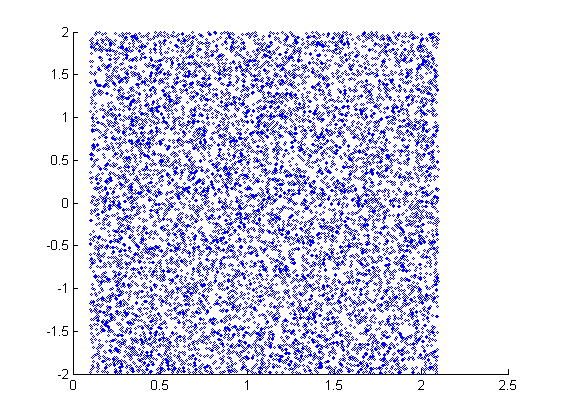
\includegraphics[width=1\textwidth]{Figs/col_m1_v1.png}
                %\caption{}
                %\label{fig:mom1}
        \end{minipage}%
%
%\hspace{20mm}
\begin{minipage}[b]{\nn\textwidth}
                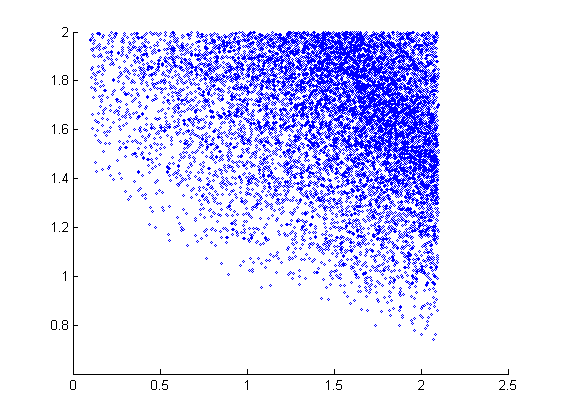
\includegraphics[width=1\textwidth]{Figs/col_m1v1_p3.png}
                %\caption{}
                %\label{fig:mom2}
        \end{minipage}%
\begin{minipage}[b]{\nn\textwidth}
                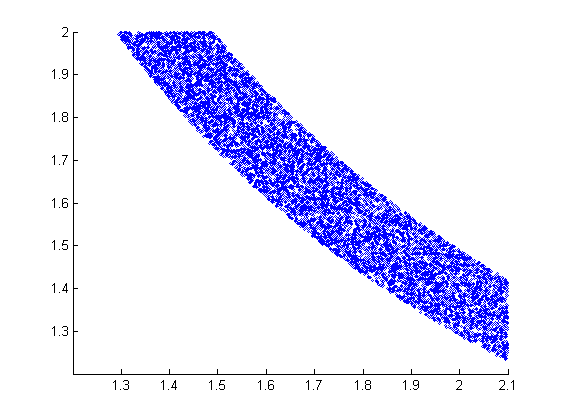
\includegraphics[width=1\textwidth]{Figs/col_m1v1_when_p_is_3_and_v2_is_0_dot_2.png}
                %\caption{}
                %\label{fig:mom2}
        \end{minipage}%
\hspace{4mm}
%\\
\begin{minipage}[b]{\nn\textwidth}
                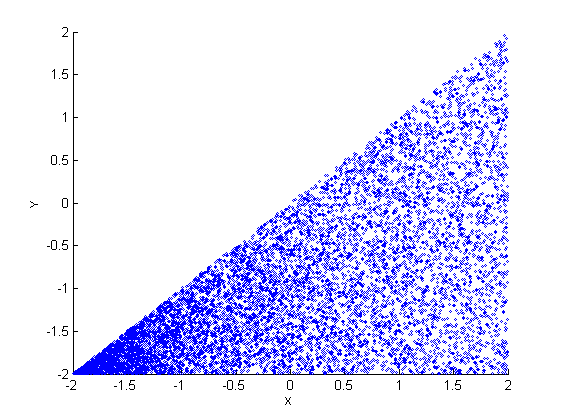
\includegraphics[width=1\textwidth]{Figs/col_v1v2.png}
                %\caption{}
                %\label{fig:mom2}
        \end{minipage}%
\begin{minipage}[b]{\nn\textwidth}
                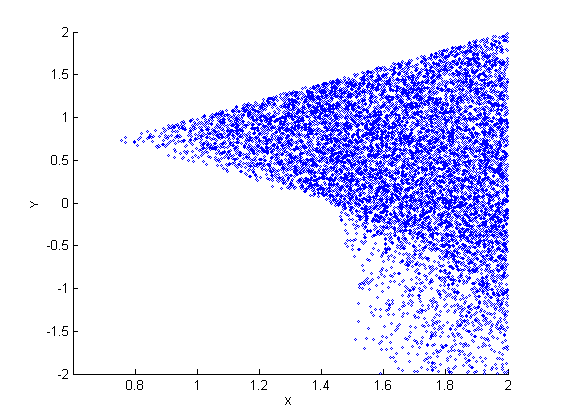
\includegraphics[width=1\textwidth]{Figs/col_v1v2whenPis3.png}
                %\caption{}
                %\label{fig:mom2}
        \end{minipage}%
\begin{minipage}[b]{\nn\textwidth}
                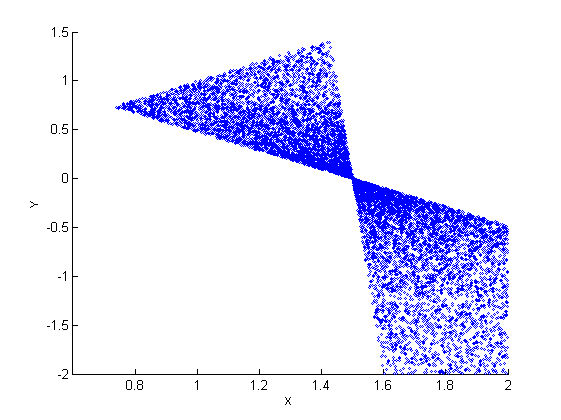
\includegraphics[width=1\textwidth]{Figs/colV1V2givenPis3M1is2.png}
                %\caption{}
                %\label{fig:mom2}
        \end{minipage}%
\end{center}
\vspace{-1mm}
\caption{\footnotesize
prior/posterior joint distributions of pairs of random variables in the \emph{collision} example. 
(a) $\pr(M_1, V_1)$,
(b) $\pr(M_1, V_1 \, | \, P_3 = 3)$,
(c) $\pr(M_1, V_1 \, | \, P_3 = 3, V_2 = 0.2)$,
(d) $\pr(V_1, V_2)$,
(e) $\pr(V_1, V_2 \, | \, P_3 = 3)$,
(f) $\pr(V_1, V_2 \, | \, M_1 =2, P_3 = 3)$
using rejection sampling on the reduced dimension model.
} 
\label{fig:mom}
%\vspace{-4mm}
\end{figure*}
%%%%%%%%%%%%%%%%%%%%%%%%%%%%%%%%%%%%%%%%%%%
\begin{figure*}
\begin{center}
%\vspace{-1mm}
\begin{minipage}[b]{\nn\textwidth}
                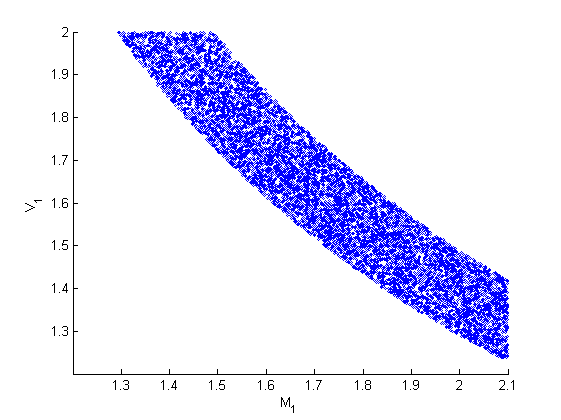
\includegraphics[width=1\textwidth]{Figs2/col_c_gibbs10000.png}
                %\caption{}
                %\label{fig:mom2}
        \end{minipage}%
\begin{minipage}[b]{\nn\textwidth}
                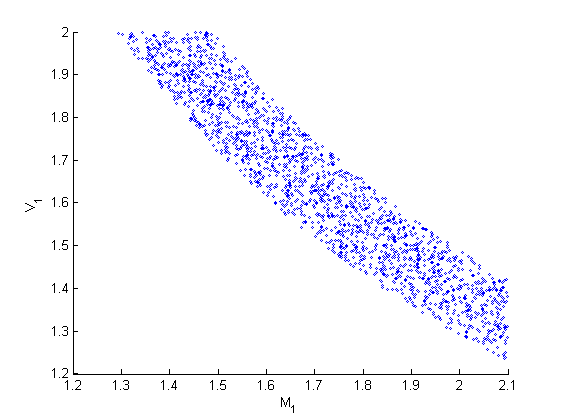
\includegraphics[width=1\textwidth]{Figs2/col-c-mh-10000_08.png}
                %\caption{}
                %\label{fig:mom2}
        \end{minipage}%
\begin{minipage}[b]{\nn\textwidth}
                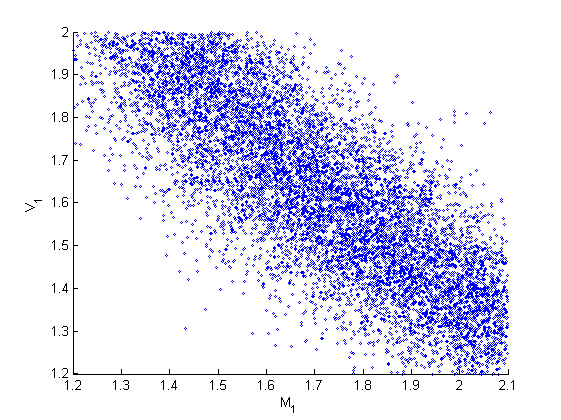
\includegraphics[width=1\textwidth]{Figs2/col_c_stan10000_02.png} % n 0.2
                %\caption{}
                %\label{fig:mom1}
        \end{minipage}%
\begin{minipage}[b]{\nn\textwidth}
                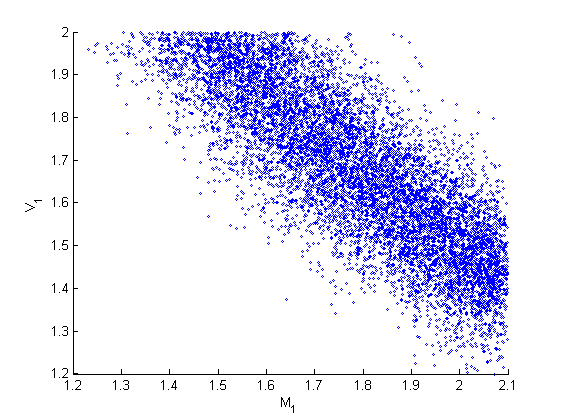
\includegraphics[width=1\textwidth]{Figs2/col_c_stan_10000_000001.png} %n 0.00001
                %\caption{}
                %\label{fig:mom2}
        \end{minipage}%
	\begin{minipage}[b]{\nn\textwidth}
                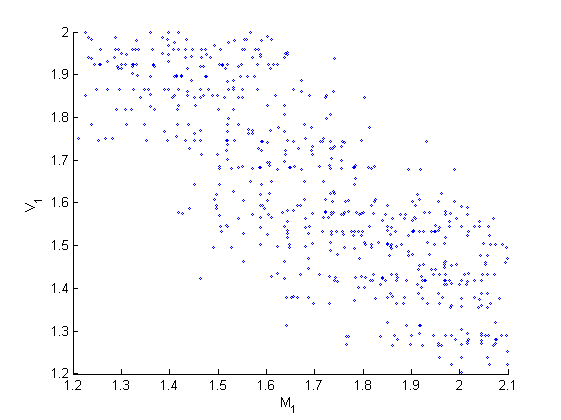
\includegraphics[width=1\textwidth]{Figs2/col_c_ang10000_02_001.png}
        \end{minipage}%
\begin{minipage}[b]{\nn\textwidth}
                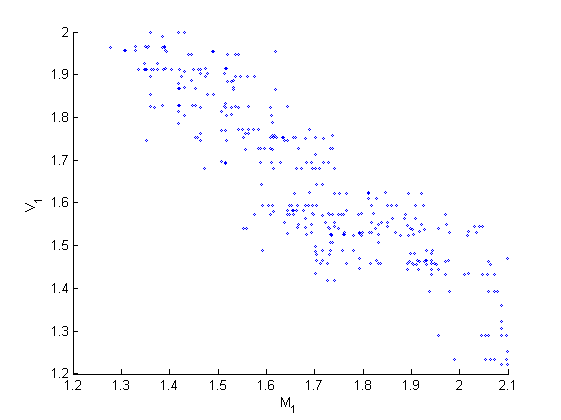
\includegraphics[width=1\textwidth]{Figs2/col_c_ang_10000_01_001}
        \end{minipage}%
\end{center}
\vspace{-1mm}
\caption{\footnotesize
10000 samples taken from the distribution Fig.~(\ref{fig:mom}-c)
using (a) Symbolic Gibbs sampler and(b) MH with \emph{proposal variance} 0.8 
on the reduced-dimension model as well as  
(c) Hamiltonian Monte Carlo (Stan) with a measurement error variance 0.2, 
, (d) and 0.00001 as well as Anglican implementation of RDB alg. with 
parameters (e)
%$V_2$ and $P_3$ observation noise variance 
$\sigma^2_{V_2} = 0.01$, $\sigma^2_{P_3} = 0.2$ and 
(f) $\sigma^2_{V_2} = 0.01$, $\sigma^2_{P_3} = 0.1$
without reducing the dimensionality.
}
\label{fig:mom2}
%\vspace{-4mm}
\end{figure*}

%%%%%%%%%%%%%%%%%%%%%%%%%%%%%%%%%%%%%%%%%%%%%%%%%%%%%%%%
\begin{figure}
\centering
%\begin{minipage}[b]{0.33\textwidth}
     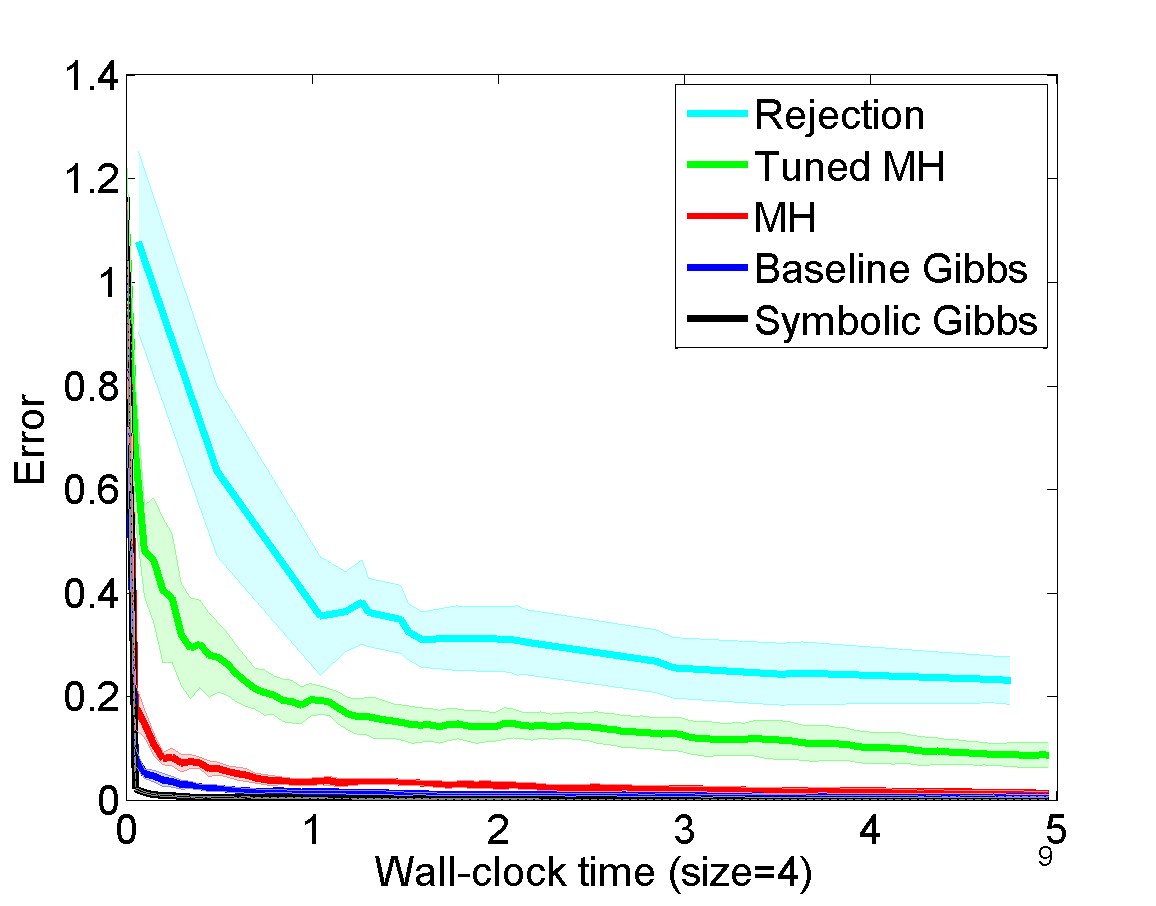
\includegraphics[width=0.8\linewidth, height=125pt]
{Figs/plots/collision/err-vs-time__param4-shaded.pdf}
   %  \caption{}
%\label{fig:collision-err-vs-time4}
%\end{minipage}
%%%
%\begin{minipage}[b]{0.33\textwidth}
 %    \includegraphics[width=1\linewidth, height=120pt]
%{Figs/plots/collision/err-vs-time__param30-shaded.pdf}
 %    \caption{}
%\label{fig:collision-err-vs-time30}
%\end{minipage}
%\begin{minipage}[b]{0.33\textwidth}
      \caption{Error %(expected value of the difference between estimated mean vector and the ground truth vector) 
as a function of wall clock time (ns) for the generalized collision problem () 
(a) for 4 colliding objects (8 stochastic variables in total since each object has a distribution over its mass and its velocity) and (b) 30 colliding objects (60 stochastic variables)
using different MCs. Note that in (b), rejection sampling has not been able to take any sample.}
      %\label{fig:dummy}
 %   \end{minipage}
\end{figure}

%%%%%%%%%%%%%%%%%%%%%%%%%%%%%%%%%%%%%%%%%%%%%%%%%%%%%%%%
\begin{figure*}
\label{fig:errVtimeSizeFixed}
\begin{center}
%\vspace{-1mm}
\begin{minipage}[b]{0.33\textwidth}
 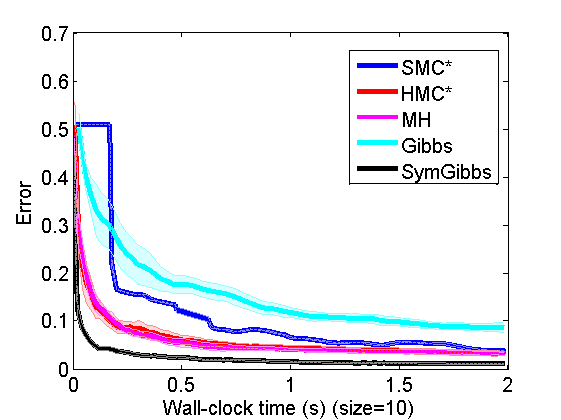
\includegraphics[width=1\linewidth, height=120pt]{plots/collision/collisionErrVsTimeInSize10.png}
\caption{generalized collision problem}
\label{fig:err-threshold-vs-size-collision}
\end{minipage}
%
\begin{minipage}[b]{0.33\textwidth}
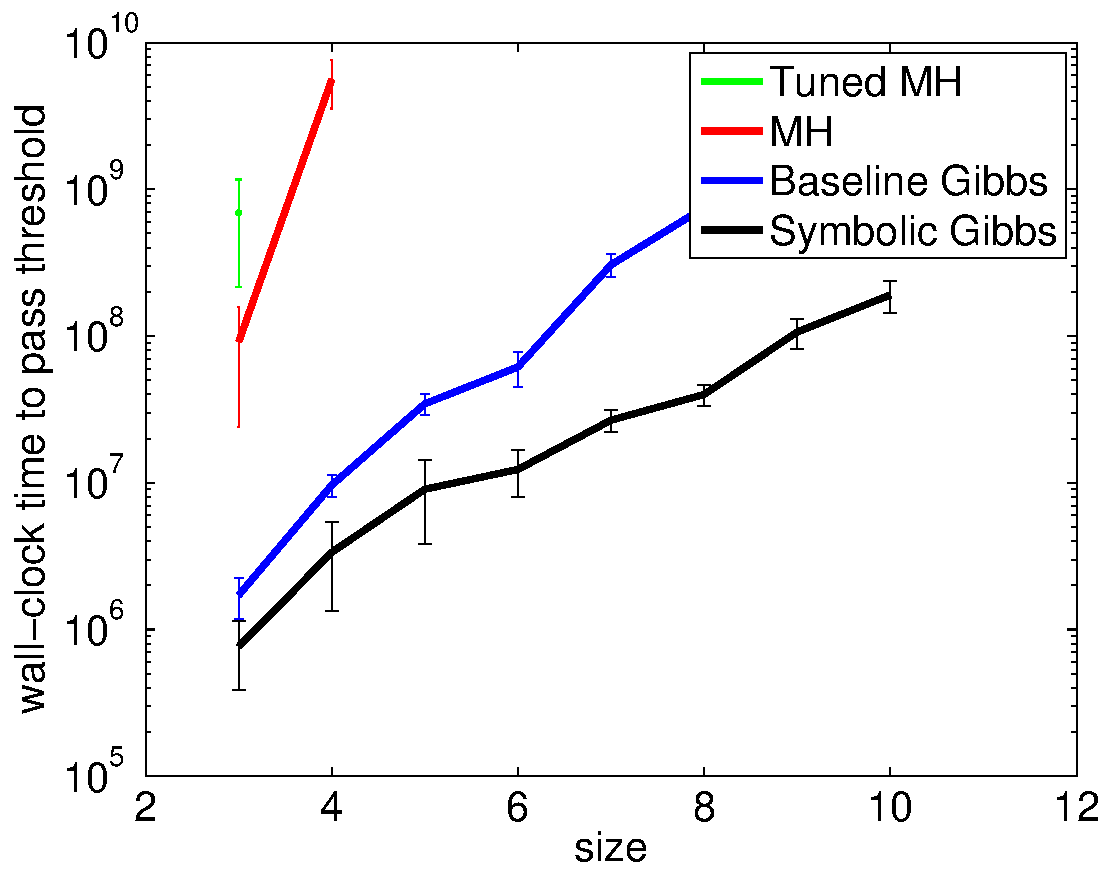
\includegraphics[width=1\linewidth, height=120pt]{Figs/plots/fermentation/time_vs_param-errorbar.pdf}
\caption{power transmission line problem}
\label{fig:err-threshold-vs-size-alc}
\end{minipage}
\begin{minipage}[b]{0.33\textwidth}
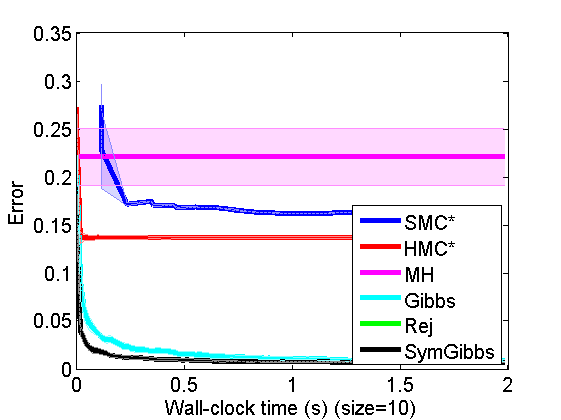
\includegraphics[width=1\linewidth, height=120pt]{plots/conductance/con_err_vs_time_size10.png}
\caption{reduced mass problem}
\label{fig:err-threshold-vs-size-circuit}
\end{minipage}
\end{center}
\caption{Wall-clock time (ns) to pass a fixed error threshold vs. the GM size, for experiments 2 to 4...TODO.}
\end{figure*}

%%%%%%%%%%%%%%%%%%%%%%%%%%%%%%%%%%%%%%%%%%%%%%%%%%%


%%%%%%%%%%%%%%%%%%%%%%%%%%%%%%%%%%%%%%%%%%%%%%%%%%%%%%%%
\begin{figure*}
\begin{center}
%\vspace{-1mm}
\begin{minipage}[b]{0.33\textwidth}
 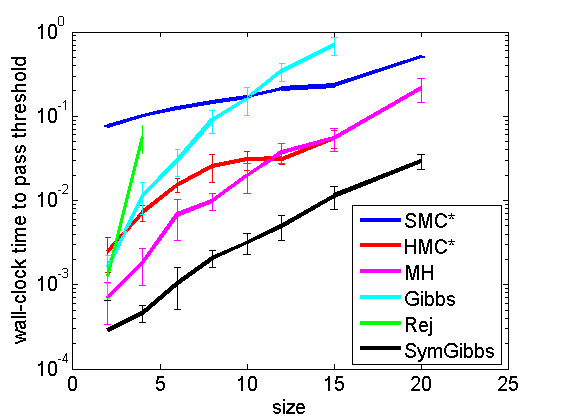
\includegraphics[width=1\linewidth, height=120pt]{plots/collision/collisionTimeVsSize.png}
\caption{generalized collision problem}
\label{fig:err-threshold-vs-size-collision}
\end{minipage}
%
\begin{minipage}[b]{0.33\textwidth}
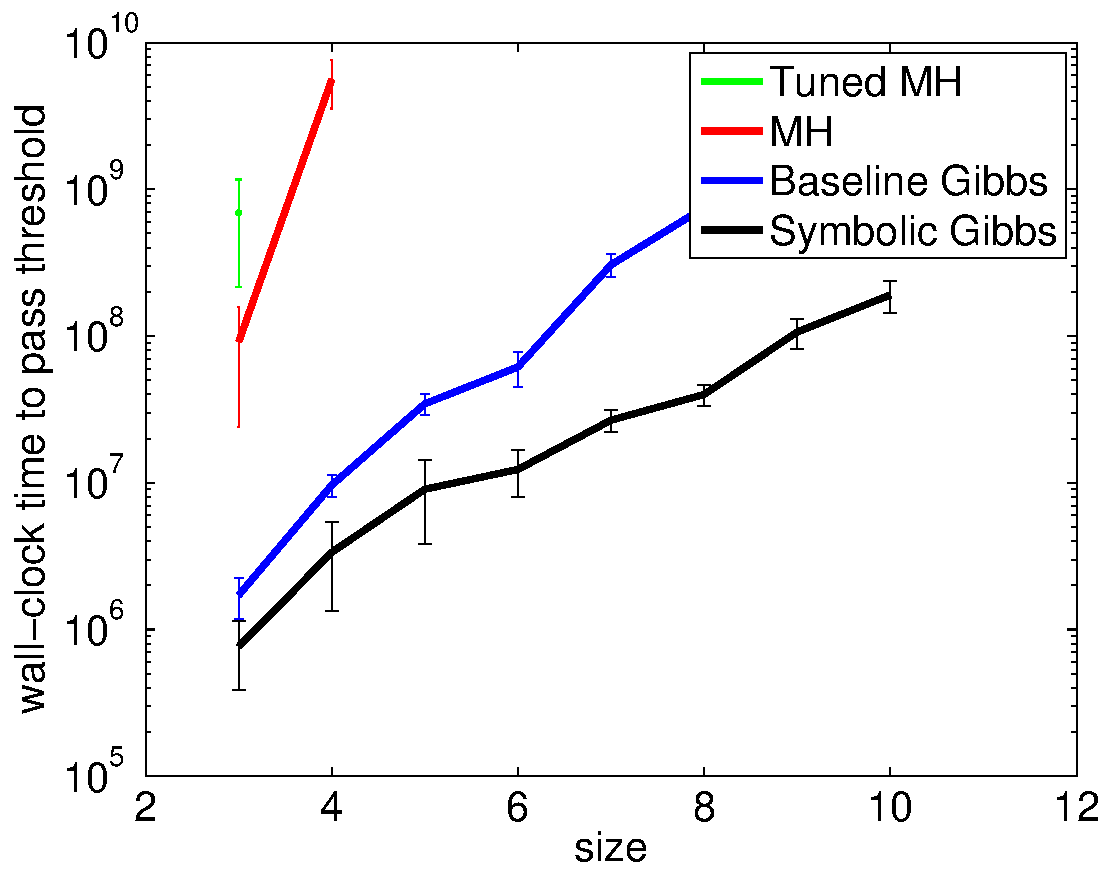
\includegraphics[width=1\linewidth, height=120pt]{Figs/plots/fermentation/time_vs_param-errorbar.pdf}
\caption{power transmission line problem}
\label{fig:err-threshold-vs-size-alc}
\end{minipage}
\begin{minipage}[b]{0.33\textwidth}
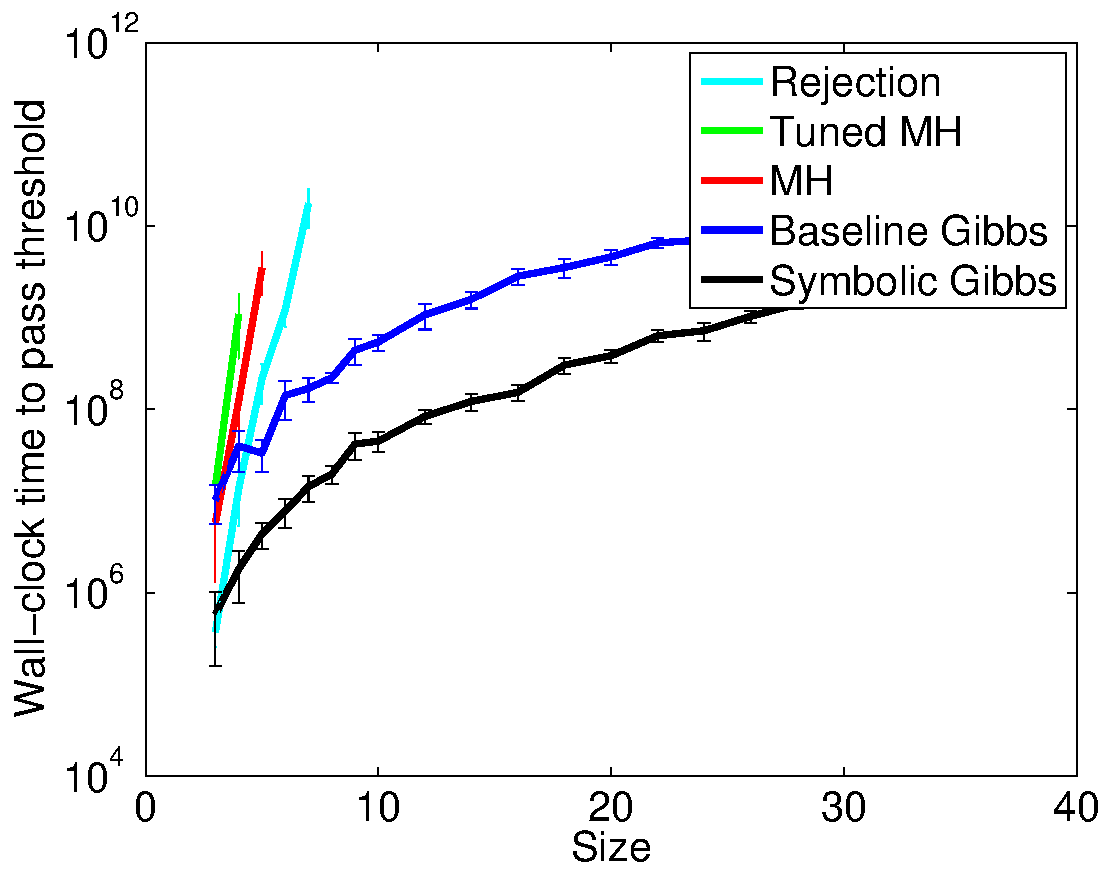
\includegraphics[width=1\linewidth, height=120pt]{Figs/plots/circuits/time_vs_param-errorbar.pdf}
\caption{reduced mass problem}
\label{fig:err-threshold-vs-size-circuit}
\end{minipage}
\end{center}
\caption{Wall-clock time (ns) to pass a fixed error threshold vs. the GM size, for experiments 2 to 4.}
\end{figure*}

%%%%%%%%%%%%%%%%%%%%%%%%%%%%%%%%%%%%%%%%%%%%%%%%%%%%%%%%
%%%%%%%%%%%%%%%%%%%%%%%%%%%%%%%%%%%%%%%%%%%%%%%%%%%%%%%%
\section{Literature review}
\label{sect:literature.review}
\section{Experimental Results}
\label{sect:experimental.results}
{\color{green}As mentioned, conditioning on deterministic constraints lead to posterior masses positioned  on submanifolds and transformations that are required for dimension reduction
often end in distributions which are highly piecewise and multimodal.
This class of distributions is intrinsically different from the smooth, bell-shaped distributions often studied in the literature. }
By carrying on four experiments we are interested in addressing the following questions: 

(a) Conditioned on hard constraints, how do posteriors look like? %(at least in lower dimensions where they can be effectively visualized)?
(b) In terms of convergence to ground truth, how do MCMC methods perform on such models? 
(c) How does approximation of observed determinism via adding noise to the observation affects the sampling convergence rate? 

\textbf{Experiment 1.} In our first experiment, we generate the posterior associated with our running example (\emph{collision model})
and plot the particles for different queries and evidence.%\footnote{We have repeated the experiment for different MCMC methods and have made sure they generate same patterns.}
The results, as depicted in the telltale plots of Figure~\ref{fig:mom}, reveal the nature of the problem tackled in this paper.
They show that even in the presence of a single deterministic constraint, 
a simple prior can transform into complicated posteriors in the form of piecewise and multimodal functions that do not resemble any family of 
probability densities studied in the literature so far. It can also be seen that more evidence generally lead to more complicated posteriors.
%The reason is that more evidence lead to more difference between the dimensionality of the non-transformed posterior submanifold and the dimensionality of the random variable space increases.
The true posteriors are approximated by 10000 particles generated by rejection sampling -- an unbiased mechanism that is functional in low dimensions as is the case of this experiment. 

To study the performance of other sampling methods, we test different MCMC algorithms on the distribution of Fig.~\ref{fig:mom}-c.
Figure~\ref{fig:mom2}-a shows that Gibbs sampling (either symbolic or baseline) on the {\color{green} reduced-dim} model generates results that are not distinguishable from the output of rejection sampling.
10000 samples generated by MH on the same model may seen  sparse (see Fig.~\ref{fig:mom2}-b) since many samples are returned multiple times leading to low effective sample size.

In the remained figures, samplers are taken via adding normal noise to the determinism rather than reducing the dimensionality.
Figures~\ref{fig:mom2}-c, \ref{fig:mom2}-d
correspond to Hamiltonian MCMC (using Stan framework) with different noise variance 0.2 and 0.01 respectively. despite the high difference between these parameter values, it can be seen that the end results are not significantly different. We conjecture that this may be due to
an internal parameter overriding mechanism in Stan to prevent near-deterministic MCMC issues. 
Finally, in Figures~\ref{fig:mom2}-c, \ref{fig:mom2}-d, the same posterior is modeled by Anglican \cite{wood2014new}.
Anglican is a probabilistic programming language with a syntax that (at least in the current version) promotes adding noise to any kind of observed variable regardless if it is deterministic 
(e.g. $P_3$) or stochastic (e.g. $V_2$). 
We use normal noise variances $0.01$ for observed variable $V_3$ and $0.2$ for observed variables $V_2$ and $P_3$ respectively.
We tested the algorithms supported by Anglican:
 sequential
Monte Carlo (SMC) \cite{wood2014new},
Particle-Gibbs (PGibbs) (a variation of Particle-MCMC\cite{andrieu2010particle}) 
and a variation of MH introduced in \cite{wingate2011lightweight} and named \emph{random database} (RDB) in \cite{wood2014new}.
Due to existence of multiple noisy observations, in terms of size and accuracy of the effective samples, the performance of all three algorithms were low. The best performance was due to RDB which is plotted. 
 
%In the second to fourth experiments, we study the role of the size of graphical model on the performance of MCMC methods.\\

\textbf{Experiment 2.} In the second experiment,
we study the role of model size on the performance of MCMC methods by generalizing the collision example to a case where $n$ objects 
collide. The difference is that we omit the sequential dependencies of velocities s.t.\ all $V_i$ and $M_i$ share a same uniform prior $U(0.2, 2.2)$ and the constraint is $\sum_{i=1}^n{M_i V_i} = P$. By this modification, the GM becomes symmetric and enables us to compute the posterior ground truth mean values manually\footnote{An alternative would be relying on \emph{MCMC convergence diagnostics} methods \cite{cowles1996markov}. The latter methods however, could produce misleading results in case MCMCs do not converge to the ground truth, a scenario that for highly complex posteriors is not improbable.}%end footnote
:
\begin{equation}
\label{e:col.GT}
M^* = V^* = \left(\frac{P}{n}\right)^{0.5}
\end{equation}
conditioned on $P = 1.5 n$, all masses $M_i$ and velocities  $V_i$ are queried. 
The tested algorithms running on the reduced-dim posterior are: 
symbolic Gibbs (see Section~\ref{sect:symbolic.gibbs}), 
baseline Gibbs (CDF computation per sample), 
%MH (Metropolis-Hastings tuned manually), 
MH automatically tuned %to reach the acceptance rate of 0.234 
after \cite{roberts1997weak})\footnote{
\label{foot:tuning}
200 {\color{green} equidistant} proposal variances in the interval $(0, 0.1]$ are tested by taking 100 samples using each and  
choosing the proposal variance for which the acceptance rate is closer to 0.24.
} and rejection sampling.
Among the samplers that add noise to determinism, {\color{green}(soften determinism(?))} 
Stan's Hamiltonian MCMC with observation noise parameter 
$\sigma_P = 0.05$ and Anglican's SMC with noise parameter $0.1$ are plotted.\footnote{
Performance of PGibbs (and RDB) have been often slightly (resp. much) poorer than SMC.
For readability of the plots, these results are not shown. 
} 
The noise variance parameters are chosen manually trying to maximize the convergence rate.
The other parameters are Stan and Anglican's default setting.

By (\ref{e:col.GT}), $a_k$, the average  of $k$-th sample vector $\bvec{s}^{(k)}$,
is expected to be $1.5^{0.5}$;   
therefore, as the overall sampling error measure, 
%$\mathbb{E}[|{\xi} - {\xi}^*|]$ 
$\mathbb{E}[|\bvec{a} - \bvec{a}^*|]$ is computed where
$\bvec{a}$ is the vector of $a_k$ (for $k$ ranges be the number of taken samples) and all entries of vector $\bvec{a}^*$ are 1.5.

For each algorithm 15 Markov chains are run and 
at consecutive time slots, their corresponding point-to-point means and standard errors are computed. 
Figure~\ref{fig:errVtimeSizeFixed}.a 
illustrates these latter results for the model of symmetric collision of 10 objects (size=10).\footnote{
Note that the dimensionality of the original space is 20 (since each object is associated with a mass and velocity random variable). Conditioned on the total momentum, reduced-dim space is 19D and algorithms that add noise to the observation, deal with  a 21D space.
} 

We repeated the experiment for different model sizes but for the sake of space restrictions, we do not depict each plot individually.
Instead we provide a single plot that summarizes the overall behavior of each sampler w.r.t.\ the model size.
We notice that after a particular threshold, the comparative performance of the samplers remains fixed.
Therefore, in Figure ???, for each sampler the (wall-clock) time (s) to reach a sampling error threshold (average) equal to 0.3 is plotted vs the model size.\footnote{
If we pick the error threshold to be too low, many samplers would never reach it. If it is too high, samplers pass it prior to be comparatively stable. On collision model, the manual error threshold choice (around) 0.3 happens to provide a fair compromise between these two requirements.  
}%end footnote

  
%In the latter high-dimensional space, the rejection sampling has not been able to generate a particle. MH algorithms convergence rate is very low while the baseline Gibbs still perform well and the symbolic Gibbs performance is at least an order of magnitude better. Finally, Figure~\ref{fig:err-threshold-vs-size-collision} depicts the time to reach a fixed error threshold $T=0.2$ versus number of colliding objects. \\
%


\textbf{Experiment 3.} Finally, we repeat the former experiment on a model with a more complicated observed determinism. 

%The last experiment, with results depicted in Figure~\ref{fig:err-threshold-vs-size-circuit}, 

Consider an electrical circuit composed of $n$, $10\Omega\pm5\%$ paralleled resistors.
% with bell-shaped tolerance distributions (truncated quadratics, positive in the range $[8, 12]$). The posterior tolerance distribution is computed when 
The input current $I$ and the source voltage $V$ are observed
and the posterior distribution of resistors is required.

Here, the observation can be stated as the following deterministic constraint:
\begin{equation} 
\label{e:reduced.mass}
 \frac{1}{R_1} + \ldots + \frac{1}{R_n} = c
\end{equation}
where $c = \frac{I}{V}$.
\footnote{
Note that the equations of the form (\ref{e:reduced.mass}) (generally referred to as \emph{reduced mass}) encounter in many problems in electrical, thermal, hydraulic, or mechanical engineering domains. 
}
Due to the symmetry of the problem, the posterior ground truth mean is known:
\begin{equation*}
R_i^* = \frac{n}{c} \qquad \text{ for } i = 1, \ldots, n
\end{equation*}
We assume 
priors $\pr(R_i) = U(9.5, \, 10.5)$, 
$c = \frac{n}{10.17}$,
Stan and Anglican observation noise divergences are 
0.02 and 0.07 respectively. Other settings are as before.

Figure ?? illustrates sampling error vs time (s) for a model with 10 resistors (size =10).
It can be seen that only variations of Gibbs sampling on the reduced model converge to the ground truth (that we are certain about because of symmetry argument). 
One reason for malfunctioning of MH-based algorithms may be as follows:
As can be verified by manual computations, conditioning on 
(\ref{e:reduced.mass}) leads to high degree terms in the posterior fraction. This corresponds such highly dense spots in the distribution that can act as traps for MH based algorithms.


\begin{comment}
\textbf{Experiment 4.} Here, we repeat the former experiment for a 
monotonically decreasing \emph{Dynamic Bayesian Network}. That is, a DBN with nodes $A_1$ to $A_n$
with priors: $A_1 \sim \mathcal{U}(0, b)$ and $A_t \sim \mathcal{U}(A_{t-1}, b)$ where 
$t = 2, \ldots n$ and $b=10$ is the upper bound and the deterministic constraint is $\sum A_i = c$.
This network models a power transmission line where energy loss takes place in components $A_t$.
However, many other applications, such as development of a chemical process, share similar models.  
The measurement takes place on the difference of the expected values of two parallel Markov chains to form a symmetry with ground truth \textbf{0}.
In the plotted results (Figure~\ref{fig:err-threshold-vs-size-alc}), 
the rejection sampling MC is missing since the joint is not log-concave and does not have a constant bound required for the algorithm's \emph{envelope} 
(note that $\lim_{A_{i} \rightarrow b} \frac{1}{b - A_{i}} = 0$ ).
\end{comment}

\section{Conclusion}
\label{sect:conclusion}

We introduced piecewise algebraic graphical models that for the first time handle a large family of nonlinear deterministic restrictions, such as the physical laws, in the form of multivariate polynomial fractions. The nonlinear nature of this data leads to a new genre of posterior distributions with possible discontinuities, 
piecewise parts with nonlinear bordering hyperplanes, rapid density changes and anomalies. Our experimental results show that Gibbs sampling performs well in the presence of such unconventional densities while other Monte Carlo methods do not. We showed that in piecewise algebraic models, the univariate CDFs required for Gibbs sampling can be computed analytically and prior to the actual sampling process. Our novel sampling method, \emph{Symbolic Gibbs}, saves a significant amount of computation, improving the performance dramatically. The combination of these novel contributions should make probabilistic reasoning applicable to variety of new applications that have remained unsolvable so far.      


%*********************************************************************************************
%*********************************************************************************************
%*********************************************************************************************

% Note use of \abovespace and \belowspace to get reasonable spacing 
% above and below tabular lines. 

%\begin{table}[t]
%\caption{Classification accuracies for naive Bayes and flexible 
%Bayes on various data sets.}
%\label{sample-table}
%\vskip 0.15in
%\begin{center}
%\begin{small}
%\begin{sc}
%\begin{tabular}{lcccr}
%\hline
%\abovespace\belowspace
%Data set & Naive & Flexible & Better? \\
%\hline
%\abovespace
%Breast    & 95.9$\pm$ 0.2& 96.7$\pm$ 0.2& $\surd$ \\
%Cleveland & 83.3$\pm$ 0.6& 80.0$\pm$ 0.6& $\times$\\
%Glass2    & 61.9$\pm$ 1.4& 83.8$\pm$ 0.7& $\surd$ \\
%Credit    & 74.8$\pm$ 0.5& 78.3$\pm$ 0.6&         \\
%Horse     & 73.3$\pm$ 0.9& 69.7$\pm$ 1.0& $\times$\\
%Meta      & 67.1$\pm$ 0.6& 76.5$\pm$ 0.5& $\surd$ \\
%Pima      & 75.1$\pm$ 0.6& 73.9$\pm$ 0.5&         \\
%\belowspace
%Vehicle   & 44.9$\pm$ 0.6& 61.5$\pm$ 0.4& $\surd$ \\
%\hline
%\end{tabular}
%\end{sc}
%\end{small}
%\end{center}
%\vskip -0.1in
%\end{table}


% Acknowledgements should only appear in the accepted version. 

% In the unusual situation where you want a paper to appear in the
% references without citing it in the main text, use \nocite
%\nocite{langley00}

\bibliography{symbolic_gibbs_icml}
\bibliographystyle{icml2015}


{\color{blue}
//-------------------------------//
%\begin{itemize}
%\item Introducing  an expressive class of functions 
%(called PPFs for \emph{Polynomial-Piecewise Polynomial Fractions}) that facilitates inference in the presence of  linear/nonlinear algebraic deterministic constraints.
%\item Presenting an efficient inference method (called \emph{Symbolic Gibbs}) that matches well with the provided model and handles deterministic constraints.  
%\end{itemize}

%for inference in graphical models (such as Bayesian networks, Markov random fields, etc.).
%PPFs are piecewise polynomial fractions where the variable space is partitioned by polynomial inequalities.
%The key insight is that the algebraic constraints preserved PPF form after collapsing which immediately extends the application of PPFs to models with sophisticated deterministic algebraic constraints. 
We note that even in simple models such as \emph{collision example}, distributions can be piecewise fractional. For example:  
\[
\pr(V_2 \,|\, V_1) = \mathcal{U}(-2, V_1)
=
\begin{cases}
  \case{\scriptstyle (V_2 > -2), \, (V_2 < V_1)}{\frac{1}{V_1 + 2}}\\
 \otherwise{0}
 \end{cases}
\]

To show the critical role of nonlinear partitioning conditions in handling the algebraic deterministic constraints, 
let us solve equation~\ref{eq:moment-constraint} for a variable (e.g.\ $V_2$):
$V_2 = \frac{3 - M_1 V_1}{M_2}$) and modify $\pr(V_2 \,|\, V_1)$ by substituting $V_2$ with its the solution.
We will see that this substitution leads to $\pr(V_2 \,|\, V_1, P_3 = 3)$:
\begin{equation}
\label{e:fractional-constraint}
\begin{cases}
  \case{(\frac{3 - M_1 V_1}{M_2} > -2) , \, (\frac{3 - M_1 V_1}{M_2} < V_1)}{\frac{1}{V_1 +2}}\\
  \otherwise{0}
  \end{cases}
\end{equation}
Clearly, this transformation has created a piecewise function with non-linear partitioning conditions.

Recently, piecewise polynomials have attracted attention.
So far, piecewise polynomials with hyperrectangular, hyper-rhombus and linear partitioning constraints have been used in Bayesian networks \cite{shenoy2011inference,shenoy2012two,Sanner:12}.
%hyperrectangular-piecewise polynomials \cite{shenoy2011inference,shenoy2012two,Sanner:12},
%hyper-rhombus-piecewise polynomials \cite{shenoy2012two} and the most general so far, linear-piecewise polynomials \cite{Sanner:12} have been used for inference in Bayesian networks.\footnote{ By \emph{A-piecewise B} we refer to piecewise functions where the function value in each partition is in class \emph{B} and the conditions partitioning the space of variables are (conjunctions of functions) in class \emph{A}.}
These models can only handle linear dependencies and 
our model is more expressive than all of them. 
%This, for the first time, enables probabilistic inference be carried on a large domain of interesting and new  applications.  

....


}%end blue
\end{document} 


% This document was modified from the file originally made available by
% Pat Langley and Andrea Danyluk for ICML-2K. This version was
% created by Lise Getoor and Tobias Scheffer, it was slightly modified  
% from the 2010 version by Thorsten Joachims & Johannes Fuernkranz, 
% slightly modified from the 2009 version by Kiri Wagstaff and 
% Sam Roweis's 2008 version, which is slightly modified from 
% Prasad Tadepalli's 2007 version which is a lightly 
% changed version of the previous year's version by Andrew Moore, 
% which was in turn edited from those of Kristian Kersting and 
% Codrina Lauth. Alex Smola contributed to the algorithmic style files.  

